\documentclass[ngerman,11pt,a4paper]{report}
\usepackage[utf8]{inputenc}
\usepackage{csquotes}
\usepackage{amsmath}
\usepackage{amsfonts}
\usepackage{amssymb}
\usepackage{dsfont}
\usepackage{algorithm}
\usepackage{algpseudocode}
\usepackage[dvipsnames]{xcolor}
\usepackage{pdfpages}
\usepackage{translator}
\usepackage{babel}
\usepackage{graphicx}
\usepackage{wrapfig}
\usepackage{color,soul}
\usepackage[bottom]{footmisc}
\usepackage{float}
\usepackage[section]{placeins}
\usepackage[backend=biber,style=numeric,sorting=none]{biblatex}
\usepackage[format=hang]{caption}
\usepackage{pgfgantt}
\usepackage[export]{adjustbox}
\usepackage{multicol}
\usepackage{xurl}
\usepackage{fancyhdr}
\usepackage{pgfkeys}
\usepackage[dvipsnames]{xcolor}
\usepackage{tikz}
\usepackage{tkz-euclide}
\usepackage{pgfplots}
\pgfplotsset{compat=1.18}
\usetikzlibrary{calc,positioning}
\usepackage{hyperref}
\usepackage[acronym,automake,nomain]{glossaries}

%---------------------------------------------------------------------------------------
\makeglossaries
\addbibresource{verweise.bib}

%PageLayout
\linespread{1.2}
\usepackage[top=2.7cm, bottom=2.8cm, left=3cm, right=3cm, headheight=20pt]{geometry}
\pagestyle{fancy}
\fancyhead{}
\fancyhead[R]{\footnotesize \fancyplain{}{\textit{\leftmark}}}
\fancyfoot{}
\fancyfoot[R]{Seite \thepage}
\fancypagestyle{plain}
{%
	\fancyhf{} % clear all header and footer fields
	\fancyfoot[R]{Seite \thepage} % except the center
	\renewcommand{\headrulewidth}{0pt}
}

%Defintions
\usepackage[framemethod=TikZ]{mdframed}
\newcounter{def}[chapter]\setcounter{def}{0}
\renewcommand{\thedef}{\arabic{chapter}.\arabic{def}}
\newenvironment{Definition}[2]
{
	\refstepcounter{def}
	\mdfsetup
	{
    	frametitle=
    	{
	        \tikz[baseline=(current bounding box.east),outer sep=0pt]
	        \node[anchor=east,rectangle,fill=Green!40]
	        {\strut Definition~\thedef:~#1};
	    },
	    innertopmargin=10pt,linecolor=Green!40,
    	linewidth=2pt,topline=true,
	    frametitleaboveskip=\dimexpr-\ht\strutbox\relax
	}
	\begin{mdframed}[backgroundcolor=Green!10]\relax
	\label{#2}
}
{
	\end{mdframed}
}

%Theorems
\newcounter{theo}[chapter]\setcounter{theo}{0}
\renewcommand{\thetheo}{\arabic{chapter}.\arabic{theo}}
\newenvironment{Satz}[2]
{
	\refstepcounter{theo}
	\mdfsetup
	{
    	frametitle=
    	{
	        \tikz[baseline=(current bounding box.east),outer sep=0pt]
	        \node[anchor=east,rectangle,fill=Green!40]
	        {\strut Satz~\thetheo:~#1};
	    },
	    innertopmargin=10pt,linecolor=Green!40,
    	linewidth=2pt,topline=true,
	    frametitleaboveskip=\dimexpr-\ht\strutbox\relax
	}
	\begin{mdframed}[backgroundcolor=Green!10]\relax
	\label{#2}
}
{
	\end{mdframed}
}

%Algorithms
\floatname{algorithm}{Algorithmus}
\renewcommand{\algorithmicrequire}{\textbf{Eingabe:}}
\renewcommand{\algorithmicensure}{\textbf{Ausgabe:}}
%---------------------------------------------------------------------------------------
%New commands
\newcommand{\argmin}{\mathop{\mathrm{arg\,min}}} 		% argmin
\newcommand{\p}{\par\bigskip\noindent}					% Für Absätze
\newcommand{\acrshortmath}[1]{\text{\acrshort{#1}}}		% Für Zugriff auf Glossary in Mathe-Umgebungen

%Math-Operator
\DeclareMathOperator{\sign}{sgn}


\author{Vipin Singh}
\title{BA_Thesis}
\date{\today}

\begin{document}
	
\includepdf{deckblatt}
	  
	\begin{abstract}
		\FloatBarrier %Verhindert Fehlpositionierung von Abbildungen aus vorherigen Abschnitten
		\setcounter{page}{2}
		\phantomsection
		\addcontentsline{toc}{chapter}{Kurzfassung}
		Das Ziel der vorliegenden Arbeit ist es, Verfahren der Deflektometrie für spiegelnde und transparente Prüfoberflächen einzuführen und mathematisch zu erklären.
Der Fokus liegt darauf, mithilfe der Verfahren die Sichtprüfung für diese Oberflächen zu ermöglichen.
Dabei wird erklärt, welche Methoden im wissenschaftlichen Gebiet der Deflektometrie eingesetzt werden, um Oberflächen vollständig zu erfassen.
Zur Bearbeitung des Themas werden transparente Brillengläser und spiegelnde Keramikobjekte analysiert und mit den eingeführten Verfahren automatisiert ausgewertet.
Die Ergebnisse der Auswertung durch die eingeführten Verfahren zeigen, dass es möglich ist, Anomalien der Oberflächenkrümmung spiegelnder und transparenter Prüfobjekte, wie z. B. Pickel, Dellen, Kratzer oder Gravuren, zu erfassen.
Dadurch wird es ermöglicht, Oberflächendefekte spiegelnder und transparenter Prüfobjekte zu lokalisieren und qualitative Aussagen der Oberflächenbeschaffenheit zu formulieren.
	\end{abstract}
	    
	%Inhaltsverzeichnis
	{
		\FloatBarrier %Verhindert Fehlpositionierung von Abbildungen aus vorherigen Abschnitten
		\setcounter{page}{3}
		\phantomsection
		\addcontentsline{toc}{chapter}{Inhaltsverzeichnis}
		\tableofcontents
	}
	    
	%Abbildungsverzeichnis
	{
		\FloatBarrier %Verhindert Fehlpositionierung von Abbildungen aus vorherigen Abschnitten
		\newpage
		\phantomsection
		\addcontentsline{toc}{chapter}{Abbildungsverzeichnis}
		\listoffigures
	}
	
	%Abkürzungsverzeichnis
	{
		\FloatBarrier %Verhindert Fehlpositionierung von Abbildungen aus vorherigen Abschnitten
		\newpage
		\phantomsection
		\addcontentsline{toc}{chapter}{Abkürzungsverzeichnis}
		\printglossary[title=Abkürzungsverzeichnis, type=\acronymtype]
		\newacronym{lr}{$l_r$}{Deflektometrische Registrierung}
\newacronym{lwidth}{$L_{width}$}{Breite des Monitorbildes in Pixel}
\newacronym{lheight}{$L_{height}$}{Höhe des Monitorbildes in Pixel}
\newacronym{lrx}{$l_{r,x}$}{Deflektometrische Registrierung der Spaltenpositionen}
\newacronym{lry}{$l_{r,y}$}{Deflektometrische Registrierung der Zeilenpositionen}
\newacronym{d}{$D$}{Definitionsmenge}
	}
	
	%Einführung
	{
		\FloatBarrier %Verhindert Fehlpositionierung von Abbildungen aus vorherigen Abschnitten
		\chapter{Einführung}
		\label{chp:einfuehrung}
		Durch die optischen Besonderheiten von spiegelnd glänzenden Oberflächen treten solche in der Industrie an vielen Stellen auf.
Speziell in der Automobilindustrie werden täglich große Karosserieflächen glänzend lackiert.
Alleine in Deutschland wurden in den Jahren von 1990 bis 2021 im Durchschnitt ungefähr 5 Millionen Personenkraftwagen pro Jahr produziert \cite{statistaPKW}.
Ein großer Teil der Fahrzeuge erhalten nach der Lackierung eine spiegelnde Oberfläche.
Solche Oberflächen müssen durch besondere Verfahren auf Defekte überprüft werden.
Dabei sorgen spekulare Reflexionen dafür, dass die Oberflächen nicht direkt, sondern über ihre Spiegelbilder der Umgebung betrachtet werden müssen. %TODO Beispielbilder?

\p
Die riesige Menge an Oberflächen macht es für die Qualitätssicherung unumgänglich die Prüfung durch automatisierte Prozesse zu integrieren.
Dabei stoßen die üblichen Verfahren der industriellen Bildverarbeitung auf ihre Grenzen, sodass neue Methoden eingeführt werden müssen.
Diese speziellen Anwendungen erfordern den Einsatz von deflektometrischen Prüfaufbauten.
In der Industrie sind solche Verfahren schon seit Längerem zur Analyse der Topographie von spiegelnden Freiformflächen etabliert.
Deflektometrische Verfahren funktionieren nach einem ähnlichen Prinzip, wie auch die Inspektion von spiegelnden Oberflächen durch Menschen. %TODO Ergänzen wie das Prinzip der Menschen funktioniert.
Das wissenschaftliche Gebiet der Deflektometrie ist auch heute noch Thema für viele Forschungsarbeiten und wird stetig weiterentwickelt.

\p
Im Rahmen der Arbeit werden spekular reflektierende Objektoberflächen unter Projektion von bekannten Mustern durch eine Kamera aufgenommen, anschließend analysiert und auf Defekte überprüft.
Welche Informationen können aus der Beobachtung von Spiegelbildern gewonnen werden?
Wie sehen allgemein anwendbare Methoden aus, um spiegelnde Oberflächen erfolgreich zu bewerten?
Das Ziel der Arbeit ist es, diese Fragen zu erforschen und aufzuklären.
Des Weiteren sollen ein Aufbau, die Ansteuerung von Beleuchtung und Kamera und die notwendige Auswertung des Bildmaterials entwickelt werden, durch welche eine Erkennung von Oberflächendefekten ermöglicht wird.
Die Umsetzung soll dabei in Form einer Softwareerweiterung für NeuroCheck erfolgen, eines sogenannten \textit{Plug-ins}.

\p
Während der Arbeit soll außerdem ein bestimmter Sonderfall genauer betrachtet werden - transparente Prüfobjekte.
Die Problematik ist dabei, dass man neben der Reflexion des Lichts, mit der Transmission zu kämpfen hat.
Dafür gibt es verschiedene Lösungsansätze wie z. B. die Auftragung einer undurchsichtigen Beschichtung.
Eine andere Möglichkeit ist eine Veränderung in dem Prüfaufbau.
Anstatt ein Muster auf das Objekt zu projizieren, kann man eine Durchlichtbeleuchtung nutzen.
Das heißt, dass man auf einem Bildschirm unter dem transparenten Prüfobjekt verschiedene Muster anzeigt.

\p
Durch die aufgenommenen Muster können Aussagen über die Oberflächenbeschaffenheit getroffen werden.
Abhängig von den verwendeten Mustern und der Auswertung sollen damit bestimmte Fehlstellen kenntlich gemacht werden.
Als Fehlstellen gelten Verformungen und Oberflächendefekte wie z. B. Dellen, Kratzer oder matte Stellen.
%TODO Weiteres schreiben im Bezug auf die nachfolgende Arbeit (vermutlich eher gegen Ende)
%Zur Detektion dieser Defekte kann man verschiedene deflektometrische Verfahren einsetzen.
%Die Verfahren können verschiedene Ergebnisse liefern, abhängig davon sind eventuell aus den Ergebnissen weitere Verarbeitungen und Auswertungen nötig.
%Im Rahmen des Projektes werden speziell die deflektometrischen Verfahren betrachtet, welche für eine Vielzahl von Anwendungen genutzt werden können.
%Nachfolgende Verarbeitungen, z. B. Detektion von Zeichen und Kratzern, werden im Rahmen des Projekts und der Bachelor-Arbeit nicht genauer behandelt.
	}
	
	%Grundlagen der Deflektometrie
	{
		\FloatBarrier %Verhindert Fehlpositionierung von Abbildungen aus vorherigen Abschnitten
		\chapter{Grundlagen der Deflektometrie}
		\label{chp:grundlagenDeflektometrie}
		Zunächst soll im folgenden Kapitel auf die Grundlagen der Deflektometrie und den Stand der Technik eingegangen werden.
Der Begriff \glqq Deflektometrie\grqq ~leitet sich aus dem lateinischen Wort \glqq deflectere\footnote{lat: deflectere: abweichen, abbiegen, ablenken}\grqq ~und dem griechischen Wort \glqq métron\footnote{griech: \textgreek{métron} : Maß, Messung}\grqq ~ab.
Somit bedeutet die Deflektometrie wörtlich übersetzt \glqq Messung der Ablenkung\grqq.
Im wissenschaftlichen Kontext wird die Deflektometrie wie folgt definiert:

\begin{Definition}{Deflektometrie}{def:deflektometrie}
	Die \textit{Deflektometrie} bezeichnet allgemein alle Methoden zur berührungslosen optischen Erfassung von Gestaltinformationen spiegelnder Oberflächen durch automatische Auswertung von Spiegelbildern bekannter Szenen. \cite{fraunhofer}
\end{Definition}

\noindent
Die Übersetzung \glqq Messung der Ablenkung\grqq ~bezieht sich dabei auf das gemessene Spiegelbild der bekannten Szene.
Die Szene wird dabei über eine Oberfläche abgelenkt und schließlich durch einen Sensor als Spiegelbild aufgenommen.
Aus dem Zusammenhang zwischen der Szene und dem Spiegelbild können Gestaltinformationen über die spiegelnde Oberfläche berechnet werden.

\begin{figure}[H]
	\centering
	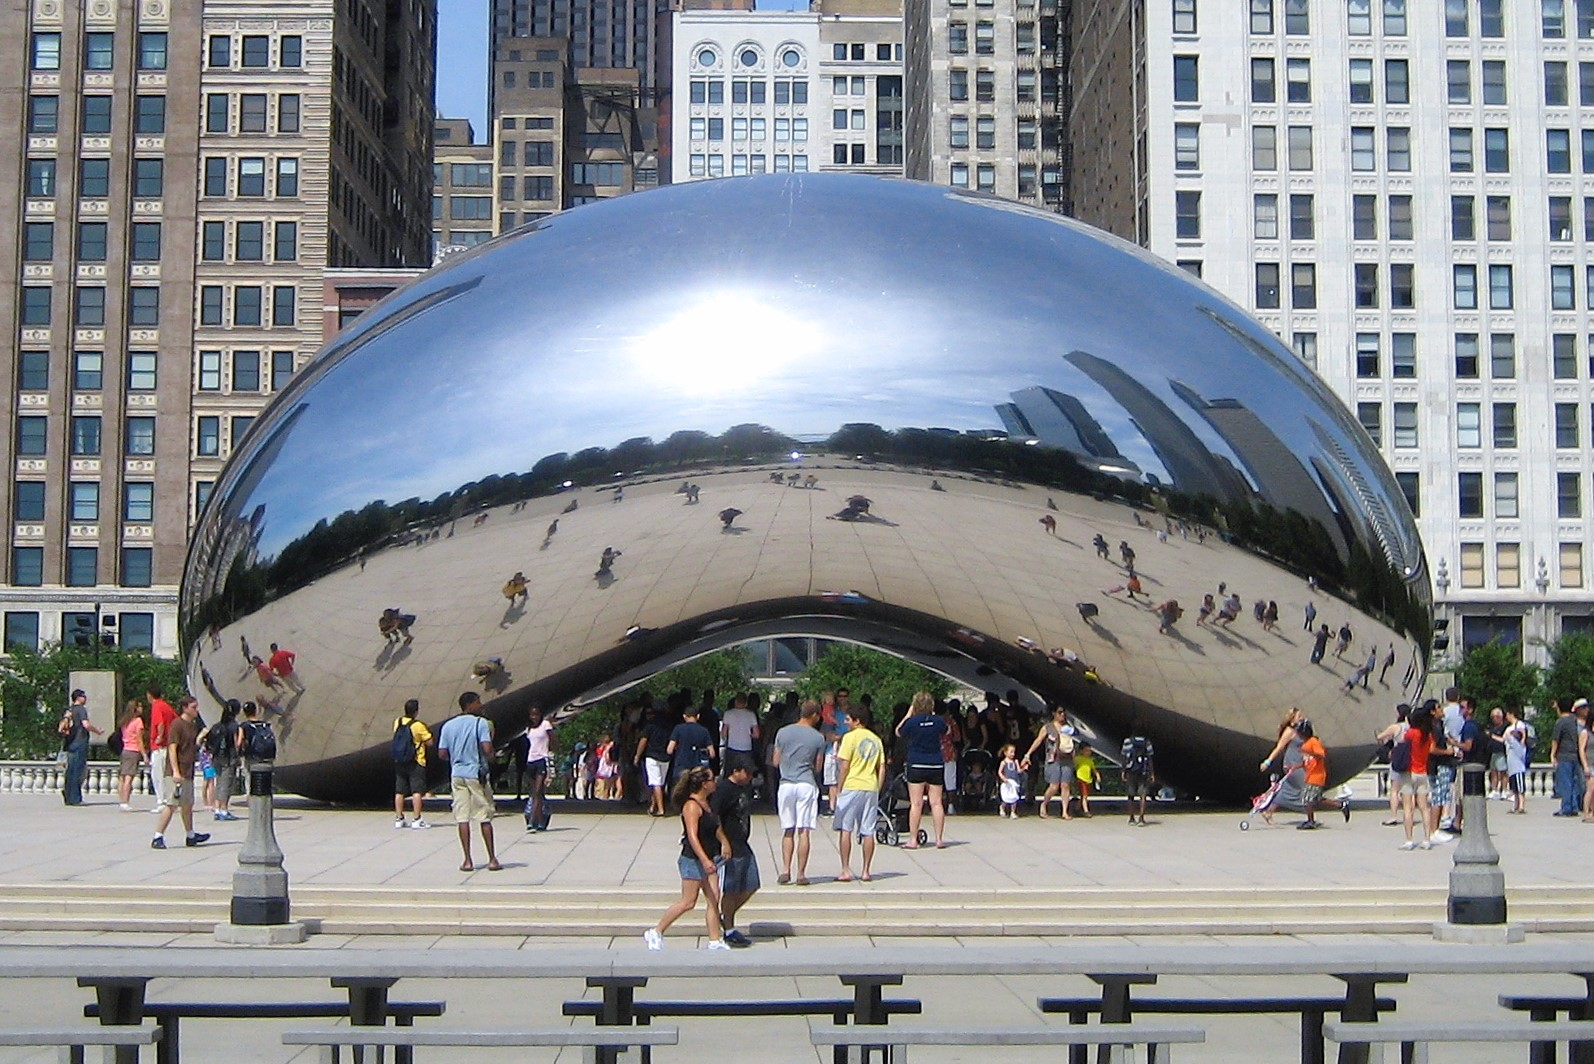
\includegraphics[width=0.55\textwidth]{02_grundlagenDerDeflektometrie/figures/cloud-gate-chicago}
	\caption[Cloud Gate Chicaog - The Bean]{Cloud Gate Chicago - The Bean \cite{cloudGateChicago}}
	\label{img:cloudGateChicago}
\end{figure}

\noindent
In Abbildung \ref{img:cloudGateChicago} erkennt man eine spiegelnde Skulptur, dessen Oberfläche ausschließlich durch die Umgebung und die Spiegelung definiert ist.
Für das menschliche Gehirn ist es zunächst nicht schwierig, die Oberflächenform zu interpretieren.
Das liegt an der Einbeziehung von Kontextinformationen.
So erkennt man z. B. über den Hintergrund und die Umgebung die Form der Skulptur.
Zusätzlich mit der Spiegelung der Szene kann man die Krümmung der Oberfläche deuten.
Wenn man den Hintergrund ausblendet, erkennt man die Schwierigkeit der Thematik (siehe Abbildung \ref{img:cloudGateMitAusschnitt}).

\begin{figure}[H]
	\centering
	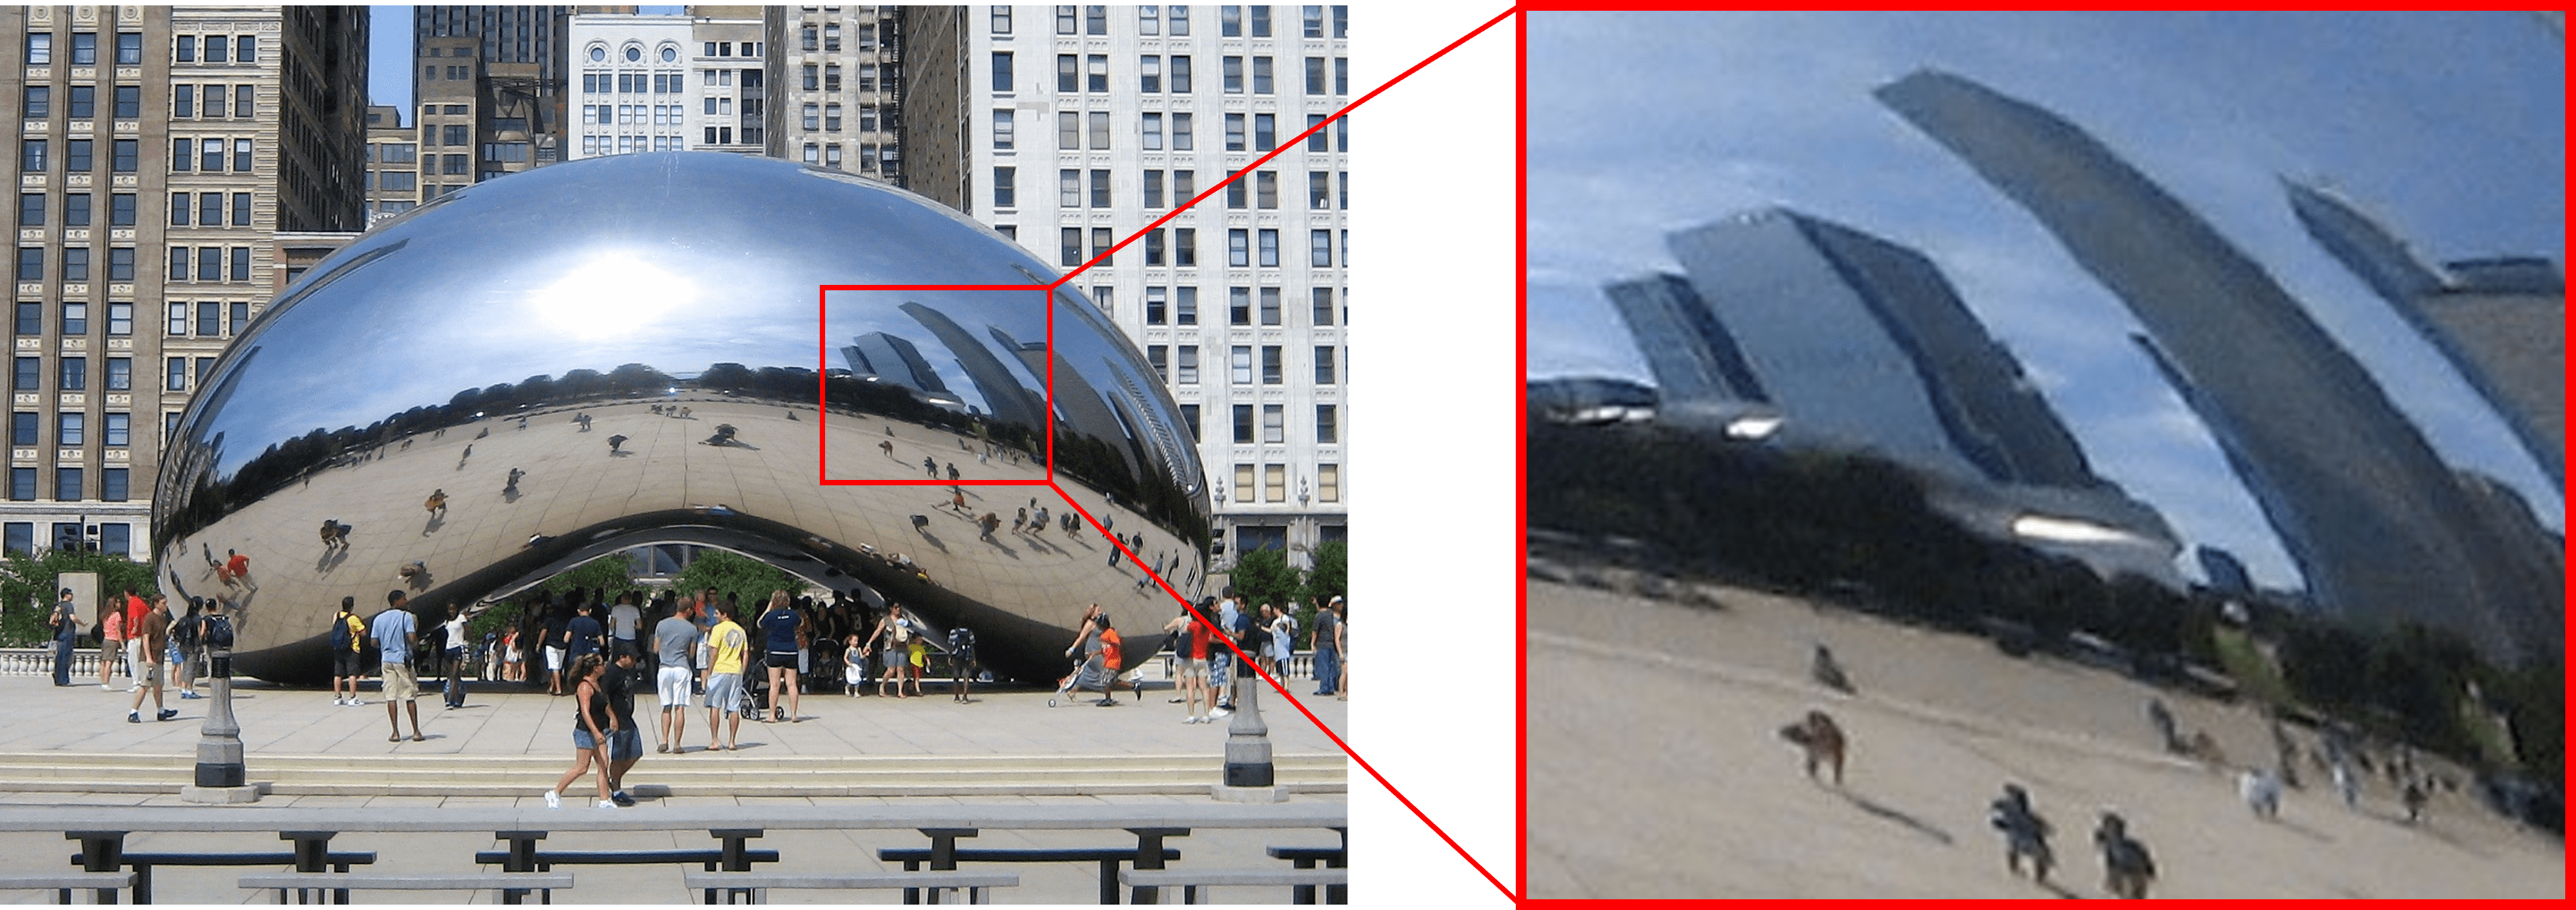
\includegraphics[width=\textwidth]{02_grundlagenDerDeflektometrie/figures/cloudGateMitAusschnitt}
	\caption[Cloud Gate mit Ausschnitt]{Cloud Gate mit Ausschnitt. \textit{in Anlehnung an} \cite{cloudGateChicago}}
	\label{img:cloudGateMitAusschnitt}
\end{figure}

\noindent
Alleine aus dem rechten Ausschnitt von Abbildung \ref{img:cloudGateMitAusschnitt} ist es schon schwieriger zu beurteilen, wie die Skulptur geformt sein könnte.
Zieht man nun Vorwissen über die gespiegelte Szene hinzu, wie z. B. das Wissen über senkrecht stehende Gebäude in Chicago, kann man Aussagen zur Gestalt der lokalen Oberfläche treffen.
Die Schwierigkeit für die automatische Auswertung ist dabei, eine eindeutige Zuordnung zwischen der Szene und dem Spiegelbild aufzustellen.
Diese und ähnliche Aufgaben, in denen Spiegelbilder analysiert werden, fallen in das Themengebiet der Deflektometrie.

\p
Die Definition \ref{def:deflektometrie} öffnet ein großes Feld für verschiedene Verfahren und Anwendungen.
Die Verfahren der Deflektometrie sind auch heute noch Themen für viele Forschungsarbeiten.

%Spiegelnde Oberflächen
{
	\FloatBarrier
    \section{Spiegelnde Oberflächen}
    \label{sec:spiegelndeOberflaechen}
    Zunächst soll auf die zu analysierenden Oberflächen genauer eingegangen werden.
Die deflektometrischen Verfahren werden explizit für spiegelnde Oberflächen entwickelt.
Doch aus welchem Grund trifft man die Unterscheidung zwischen spiegelnden und nicht-spiegelnden Objekten?
Warum lassen sich Verfahren für diffus reflektierende Oberflächen nicht auch für spiegelnden Oberflächen anwenden?
Zur Beantwortung dieser Fragen sollte man die Eigenschaften der Oberflächen genauer betrachten.
Eine diffus reflektierende Oberfläche strahlt die auftreffenden Lichtstrahlen in viele Richtungen ab, wohingegen spekular reflektierende Oberflächen die Lichtstrahlen in eine Richtung reflektieren.
Diffus reflektierende Oberflächen werden als matt oder rau bezeichnet, weil die Lichtstrahlen auf mikroskopischer Ebene auf eine raue Oberfläche treffen.
Spekular reflektierende Oberflächen werden als spiegelnd oder glatt bezeichnet, weil die Lichtstrahlen auf mikroskopischer Ebene auf eine glatte Oberfläche treffen.
Abbildung \ref{tikz:abbGlattUndRau} zeigt diesen Zusammenhang zwischen der mikroskopischen Oberflächenbeschaffenheit und den daraus folgenden Reflexionseigenschaften.

% Abbildung: Glatte und Raue Oberfläche
{
	\begin{figure}[H]
		\centering
		\begin{adjustbox}{width=\textwidth}
	\begin{tikzpicture}[every node/.style={inner sep=0,outer sep=0}]
	
		\node [anchor=north east] (imgGlatt) at (-0.03\textwidth,0) {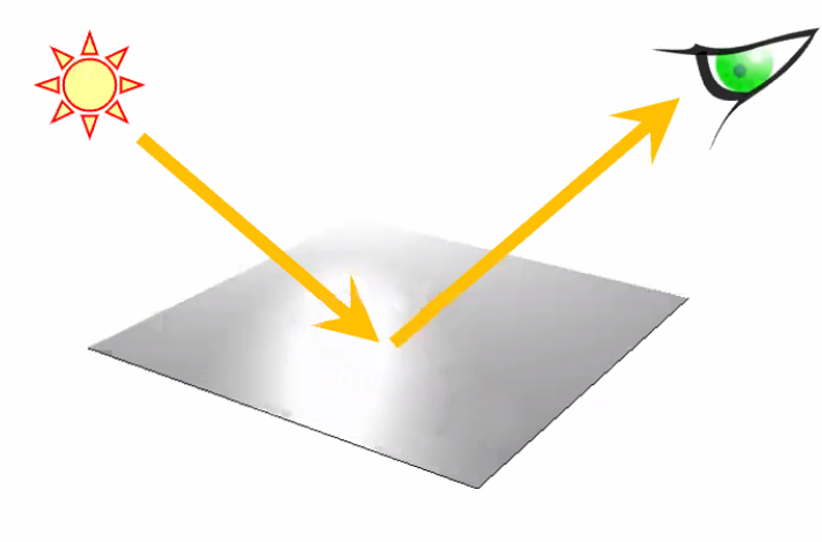
\includegraphics[width=.47\textwidth]{02_grundlagenDerDeflektometrie/spiegelndeOberflaechen/figures/spiegelnd}};
		\node [below=0.2cm of imgGlatt, align=center] {Spiegelnde Oberfläche mit glatter \\ Oberflächenbeschaffenheit};
		\node [anchor=north west] (imgRau) at (0.03\textwidth,0) {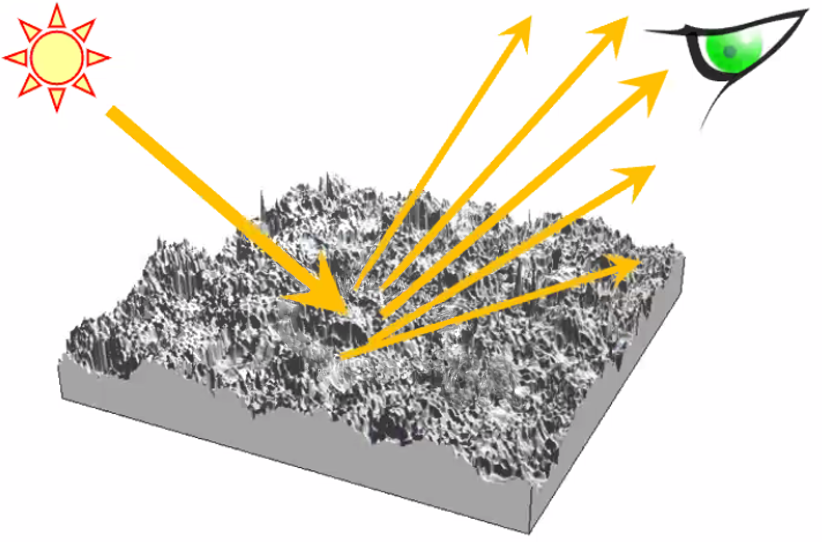
\includegraphics[width=.47\textwidth]{02_grundlagenDerDeflektometrie/spiegelndeOberflaechen/figures/rau}};
		\node [below=0.2cm of imgRau, align=center] {Matte Oberfläche mit rauer \\ Oberflächenbeschaffenheit};
		
	\end{tikzpicture}
\end{adjustbox}
\caption[Spiegelnde und matte Oberflächen]{Spiegelnde bzw. glatte und matte bzw. raue Oberflächen in ihrer mikroskopischen Oberflächenbeschaffenheit. \cite{jenaerOK}}
		\label{tikz:abbGlattUndRau}
	\end{figure}
}
%
\noindent
Durch diese unterschiedliche Reflexionsarten eignen sich für die Oberflächen unterschiedliche Szenen zur Auswertung der Krümmung.
Während spiegelnde Oberfläche ein abbildendes System der Szene darstellt, lässt sich eine Szene über die matte Oberfläche nicht durch eine Spiegelung beobachten.
Für matte Oberflächen eignet sich daher eine Projektion mit viel Licht zur Beobachtung einer Szene.
Für spiegelnde Oberflächen ist dies aufgrund der hohen Reflektivität ungeeignet, stattdessen verwendet man zur Darstellung einer Szene direkt einen Bildschirm (siehe Abbildung  \ref{tikz:abbDeflektometrieVSProjektion}).

% Abbildung: Glatte und Raue Oberfläche
{
	\begin{figure}[H]
		\centering
		\begin{adjustbox}{width=\textwidth}
	\begin{tikzpicture}[every node/.style={inner sep=0,outer sep=0}]
	
		\node [anchor=north east] (imgDeflektometrie) at (-0.03\textwidth,0) {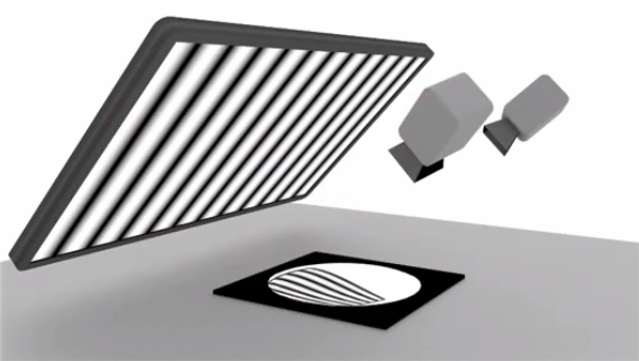
\includegraphics[width=.47\textwidth]{02_grundlagenDerDeflektometrie/spiegelndeOberflaechen/figures/deflektometrie}};
		\node [below=0.2cm of imgDeflektometrie, align=center] {Deflektometrische Verfahren für \\ spiegelnde Oberflächen};
		\node [anchor=north west] (imgProjektion) at (0.03\textwidth,0) {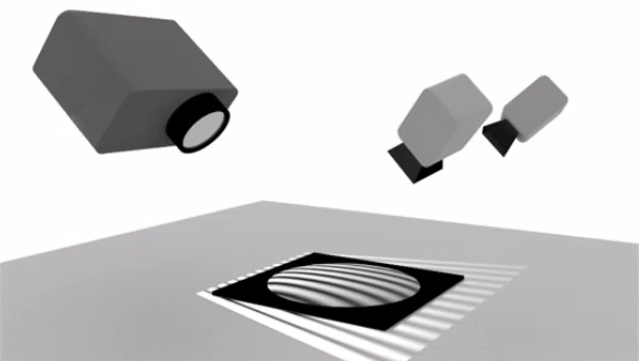
\includegraphics[width=.47\textwidth]{02_grundlagenDerDeflektometrie/spiegelndeOberflaechen/figures/streifenlichtprojektion}};
		\node [below=0.2cm of imgProjektion, align=center] {Streifenlichtprojektion für \\ matte Oberflächen};
		
	\end{tikzpicture}
\end{adjustbox}
\caption[Spiegelnde und matte Oberflächen]{Spiegelnde bzw. glatte und matte bzw. raue Oberflächen in ihrer mikroskopischen Oberflächenbeschaffenheit. \cite{jenaerOK}}
		\label{tikz:abbDeflektometrieVSProjektion}
	\end{figure}
}

\noindent
Im Vergleich erreichen beide Beleuchtungen die Aufnahme einer Szene über der Oberfläche.
Dies ist notwendig um bestimmte Aussagen über die Prüfobjekte treffen zu können.
Der wesentliche Unterschied der beiden Verfahren besteht in der Messempfindlichkeit.
Die deflektometrischen Messverfahren sind neigungssensitiv, da die Reflexion direkt von der Oberflächennormale an den auftreffenden Stellen abhängt.
Im Gegensatz dazu ist die Streifenlichtprojektion durch das Hinzufügen einer Projektionslinse ein höhensensitives Messverfahren für diffus reflektierende Objekte.
Die Oberflächenneigung selbst beeinflusst die aufgenommene Szene bei der Streifenlichtprojektion nicht sehr stark.
Durch die unterschiedliche Funktionsweise der Beleuchtungen für spiegelnde und matte Oberflächen verwendet auch unterschiedliche Verfahren zur Auswertung der Messungen.
Dennoch behandelt man eine ähnliche Fragestellung und findet somit auch Analogien in den Verfahren.

\p
Zuletzt ist es noch wichtig die Besonderheiten von transparenten Objekten zu untersuchen.
Die Oberflächen klarer transparenter Objekte sind glatt und gehören somit zur Kategorie der spiegelnden Oberflächen.
Entscheidend für die transparente Eigenschaft ist die hohe Lichttransmission solcher Objekte, d. h. die Eigenschaft das eintreffende Licht durch das Objekt durchzulassen.
Das bedeutet, dass das Licht in das Objekt eindringen und innerhalb des Objekts gebrochen und reflektiert werden kann (siehe Abbildung \ref{img:rueckseitenreflex}).

% Abbildung: Rückseitenreflex
\begin{figure}[H]
	\centering
	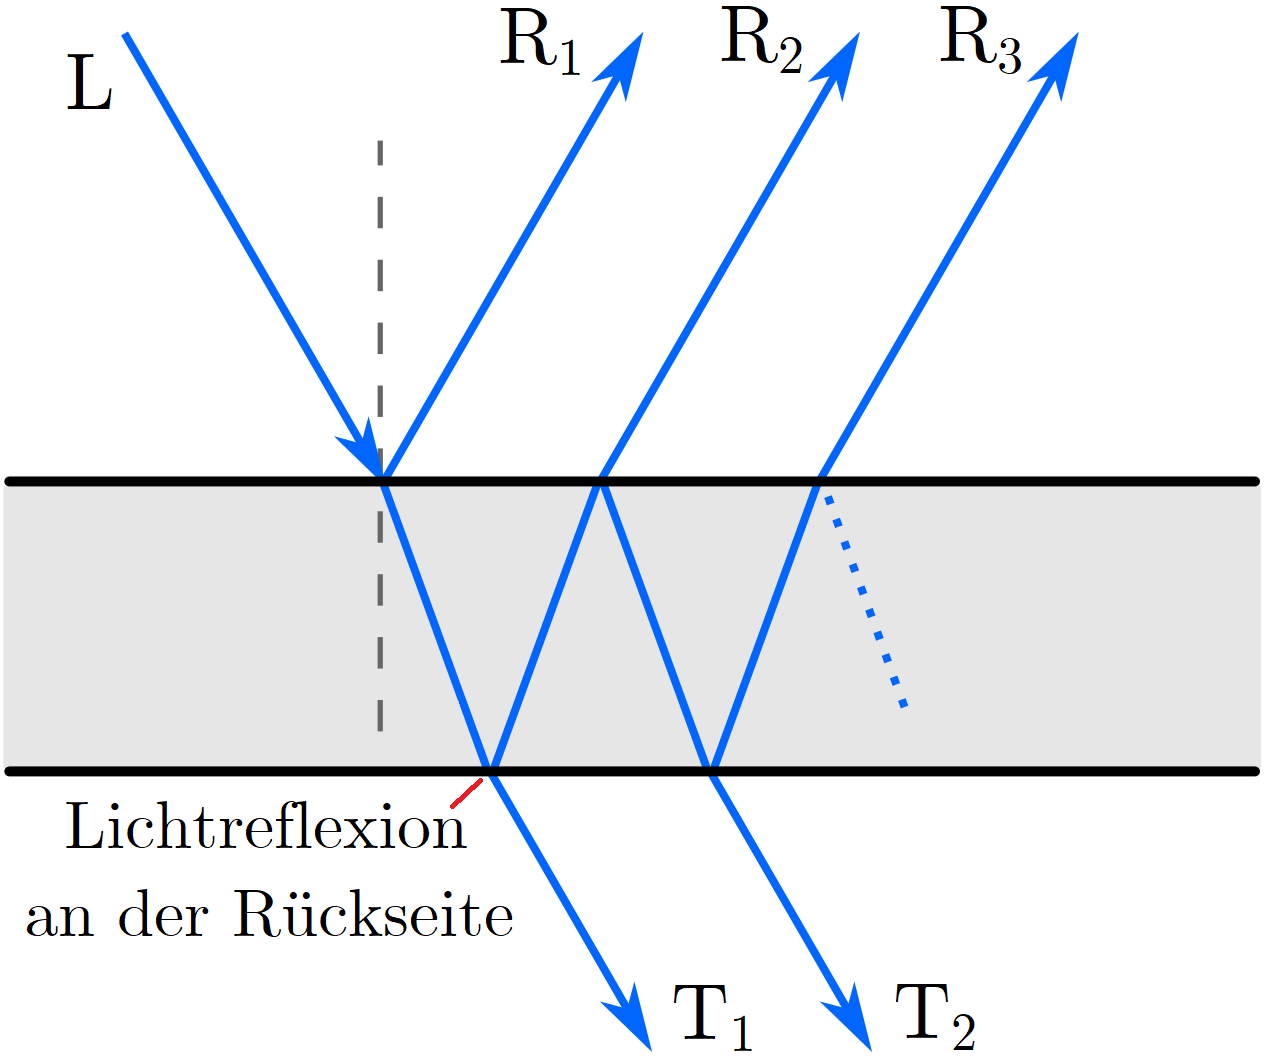
\includegraphics[width=0.4\textwidth]{02_grundlagenDerDeflektometrie/spiegelndeOberflaechen/figures/rueckseitenreflex}
	\caption[Rückseitenreflex]{Brechung und Reflexion an einem ebenen transparenten Objekt. $L$ bezeichnet den eingehenden Lichtstrahl, $R_i$ die reflektierten Lichtstrahlen und $T_i$ die transmittierten Lichtstrahlen. \cite{deflektometrieScheiben}}
	\label{img:rueckseitenreflex}
\end{figure}

\noindent
Die Lichtreflexion an der Rückseite des Objekts wird Rückseitenreflex genannt.
Dadurch entsteht im Sichtfeld eine Über\-la\-ge\-rung von einer doppelt reflektierten Szene.
Diese Über\-la\-ge\-rung sorgt für Probleme in der Auswertung der aufgenommenen Bildern.
In Abbildung \ref{img:rueckseitenreflexBeispiel} wird der Rückseitenreflex einer Glaslinse dargestellt.
Die Szene ist dabei eine Streifenbeleuchtung durch einen Bildschirm.

% Abbildung: Rückseitenreflex Beispiel
\begin{figure}[H]
	\centering
	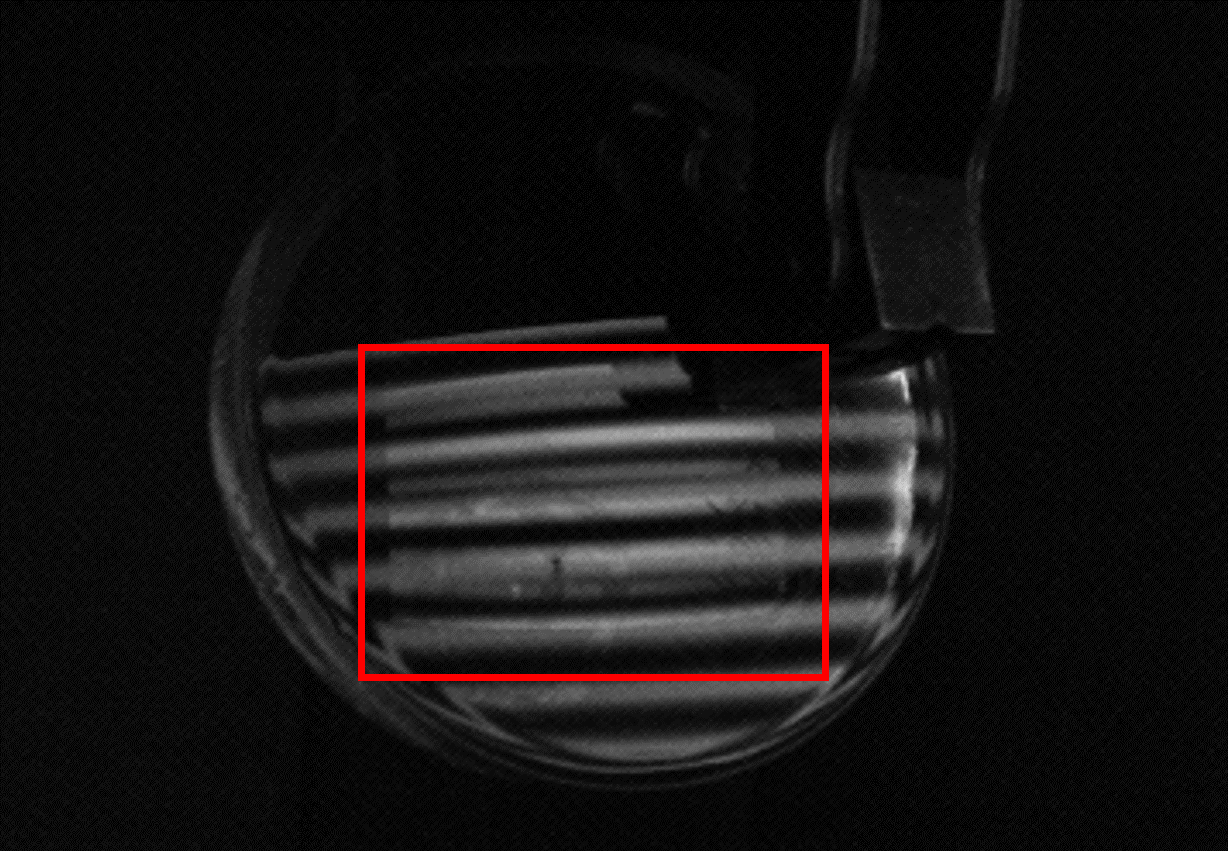
\includegraphics[width=0.5\textwidth]{02_grundlagenDerDeflektometrie/spiegelndeOberflaechen/figures/rueckseitenreflexBeispiel}
	\caption[Beispiel Rückseitenreflex]{Beispiel eines Rückseitenreflex einer transparenten Glaslinse. Im roten Rechteck erkennt man eine leichte zweite Reflexion.}
	\label{img:rueckseitenreflexBeispiel}
\end{figure}

\noindent
Den Effekt des Rückseitenreflex lässt sich durch bestimmte Verfahren, wie z. B. eine undurchsichtige Beschichtung der Oberfläche des transparenten Objekts vermeiden.
Dadurch beschädigt man aber auch die Oberfläche des untersuchten Objekts.
Andere Mög\-lich\-keiten dies zu reduzieren sind spezielle Beleuchtungen, z. B. statt LCD-Bildschirme kann man Beleuchtungen mit Lichtwellen im ultravioletten Bereich verwenden \cite{invisionUVDeflektometrie}.
Ganz umgehen kann man den Rückseitenreflex indem man keine Reflexion aufnimmt, sondern mit Durchlicht arbeitet.
Damit kommen man allerdings auch Einschränkungen einher, die bestimmte Verfahren ausschließen.

\p
Mit diesem Wissen über den Einsatz von bestimmter Beleuchtungsstrategien für spezielle Oberflächen und Objekte, kann man Verfahren beschreiben zur Analyse von spiegelnden Oberflächen.
}

%Rekonstruktion von spiegelnden Oberflächen
{
	\FloatBarrier
    \section{Rekonstruktion von spiegelnden Oberflächen}
    \label{sec:rekonstruktion}
    Das Hauptforschungsgebiet der gegenwärtigen Deflektometrie ist die Generierung von dreidimensionalen Modellen von spiegelnden Objektoberflächen.
Der Aufbau eines solchen Anwendungsfalls sieht eine Beleuchtungseinheit (z. B. einen Bildschirm), einen Sensor (z. B. eine Kamera) und ein zu untersuchendes Objekt vor.

\begin{figure}[H]
	\centering
	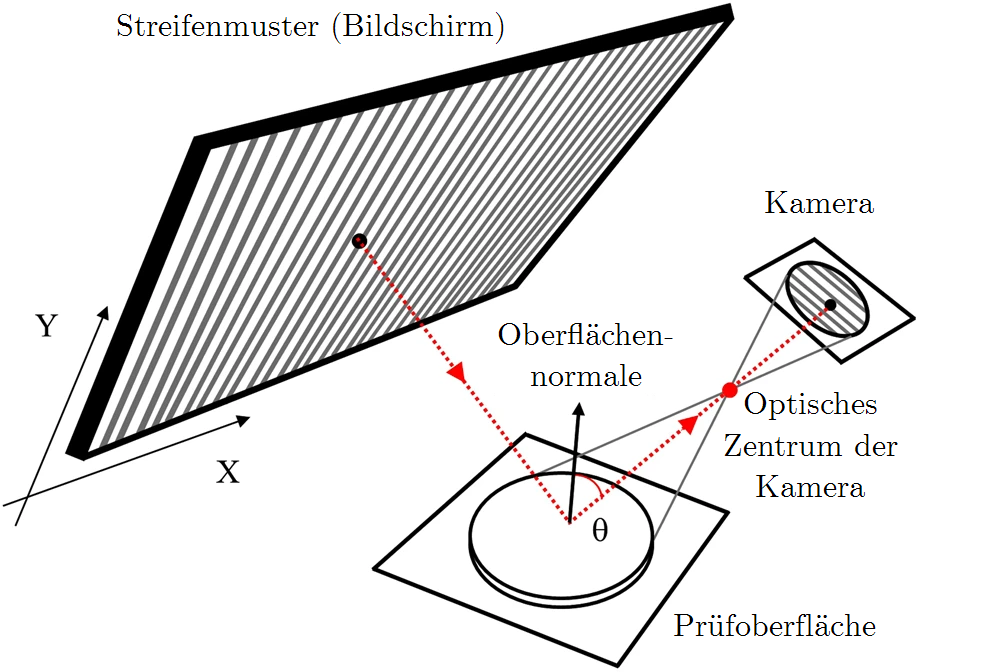
\includegraphics[width=0.7\textwidth]{02_grundlagenDerDeflektometrie/rekonstruktion/figures/nature-articel-nr1}
	\caption[Aufbau einer Deflektometrie-Prüfstation]{Aufbau einer Deflektometrie-Prüfstation. \textit{in Anlehnung an} \cite{aufbau}}
	\label{img:aufbau}
\end{figure}

\noindent
Wie in Abbildung \ref{img:aufbau} angedeutet, wird ein Muster als bekannte Szene auf ein Prüfobjekt abgebildet und anschließend von einer Kamera aufgenommen.
Das grundlegende Prinzip basiert darauf, dass jeder durch die Kamera aufgenommene Punkt des Objekts dem Punkt auf dem Bildschirm zugeordnet wird, der den Objektpunkt beleuchtet bzw. der am Objektpunkt in die Kamera reflektiert wird.
Dabei ordnet man jedem Pixel des projizierten Musters sein zugehöriges Pixel des erzeugten Musters auf dem Bildschirm zu.
Durch diese Zuordnung von Kamera- und Bildschirmpunkten lassen sich Neigungsinformationen der Oberfläche berechnen.
Dies kann durch Strahlenverfolgungen erreicht werden.
In Abbildung \ref{img:aufbau} lässt sich das über die in Rot eingezeichneten Vektoren erkennen.
Die Schwierigkeit liegt in der eindeutigen Zuordnung zwischen der Szene und dem Spiegelbild.
Hierfür gibt es verschiedene Ansätze, dies zu erreichen.
Grundlegend ist dabei die Kodierung der Objektoberfläche (siehe Definition \ref{def:kodierungOberflaeche}), damit diese durch die Kamera aufgenommen werden kann.
Die Kamera digitalisiert dann die kodierte Oberfläche zu einem oder mehreren Bildern.
Unter Berücksichtigung der Kodierung können die Bilder durch einen entsprechenden Softwarealgorithmus dekodiert werden und man erhält damit die Zuordnung zwischen der Szene und dem Spiegelbild (siehe Abbildung \ref{tikz:abbKodierungUndDekodierung}).
%
% Definition: Kodierung der Objektoberfläche
\begin{Definition}{Kodierung der Objektoberfläche}{def:kodierungOberflaeche}
	Die Abbildung einer oder mehrerer vordefinierter Szenen auf eine spiegelnde Oberfläche wird als \textit{Kodierung der Objektoberfläche} bezeichnet.
	Das Ziel ist es dabei die Punkte aus der Szene eindeutig durch eine oder mehrere Aufnahmen der Oberfläche zu identifizieren.
\end{Definition}
%
%
% Abbildung: Kodierung und Dekodierung
{
	\begin{figure}[H]
		\centering
		\begin{adjustbox}{width=\textwidth}
	\begin{tikzpicture}
	[
		rectnode/.style={rectangle, draw=red!60, fill=red!5, very thick, minimum width={3cm}, font=\small, rounded corners},
		ellipsenode/.style={ellipse, draw=green!60, fill=green!5, very thick, minimum width={3cm}, font=\small},
		calloutnode/.style={rectangle callout, draw=RoyalPurple, fill=RoyalPurple!5, text=RoyalPurple, font=\footnotesize, rounded corners},
	]

		\node[ellipsenode] (source) {Quelle};
		\node[rectnode] (encoder) [right=of source] {Kodierung};
		\node[rectnode] (channel) [below right=of encoder] {Digitalisierung};
		\node[rectnode] (decoder) [below left=of channel] {Dekodierung};
		\node[ellipsenode] (drain) [left=of decoder]{Ergebnis};		
		
		\draw[->] (source.east) -- (encoder.west);
		\draw[->] (encoder.east) -| (channel.north);
		\draw[->] (channel.south) |- (decoder.east);
		\draw[->] (decoder.west) -- (drain.east);
		
		\node[right=of channel, font=\small, align=center] (noise) {Rauschen,\\ Unschärfe};
		\draw[->] (noise.west) -- (channel.east);
		
		\node[calloutnode] (surface) [callout absolute pointer=(source.north), above=of source.east, anchor=east] {Objektoberfläche};
		\node[calloutnode] (illumination) [callout absolute pointer=(encoder.north), above=of encoder.east, anchor=east] {Beleuchtung};
		\node[calloutnode] (camera) [callout absolute pointer=(channel.30), above=of channel.east, anchor=east] {Kamera};
		\node[calloutnode] (software) [callout absolute pointer=(decoder.north), above=of decoder.east, anchor=east] {Algorithmus};
		\node[calloutnode] (result) [callout absolute pointer=(drain.north), above=of drain.east, anchor=east] {Zuordnung};
		
	\end{tikzpicture}
\end{adjustbox}
\caption[Kodierung und Dekodierung der Objektoberfläche]{Kodierung und Dekodierung der Objektoberfläche.}
		\label{tikz:abbKodierungUndDekodierung}
	\end{figure}
}

\noindent
Die Art, wie man die Informationen in den digitalen Kanal überträgt, ist entscheidend für eine gute Zuordnung.
Aus dem Grund werden sich in wissenschaftlichen Forschungsarbeiten einige Gedanken über die Kodierung der Objektoberfläche gemacht.
Auf eine Auswahl von Möglichkeiten aus dem heutigen wissenschaftlichen Stand soll im Folgenden eingegangen werden.
%
% Phasenkodierung
{
	\FloatBarrier
    \subsection{Phasenkodierung}
    \label{sub:phasenKodierung}
    Die am häufigsten eingesetzte Kodiermethode im Kontext der Deflektometrie ist die Phasenkodierung.
Dieser Ansatz wird im Themengebiet der \glqq Phasenmessenden Deflektometrie\grqq ~beschrieben.
Dabei verwendet man Streifenmuster die entlang der Ausbreitung der Streifen, den Grauwertverlauf einer trigonometrischen Funktion (z. B. Sinus- oder Kosinus-Funktion) annehmen.
Solche Muster nennt man auch sinusoidale Streifenmuster.
Die Szene bzw. der Monitor wird dabei über die Phase der Sinus-Funktion kodiert.
Das heißt, jeder Punkt auf einem Monitor, angegeben durch eine $x$- und eine $y$-Koordinate, wird durch eine Phase $\phi_x$ in $x$-Richtung und eine Phase $\phi_y$ in $y$-Richtung kodiert.
Verwendet man Streifenmuster, stellt man die Kodierung in zwei Bildern dar.
Das erste Bild kodiert die Spaltenpositionen durch die Phasen $\phi_x$ und das zweite Bild kodiert die Zeilenpositionen durch die Phasen $\phi_y$ (siehe Abbildung \ref{tikz:abbSinusoidaleStreifenmuster}).

\begin{figure}[H]
	\centering
		\input{02_grundlagenDerDeflektometrie/rekonstruktion/phasenKodierung/figures/abbSinusoidaleStreifenmuster}
		\label{tikz:abbSinusoidaleStreifenmuster}
\end{figure}

\noindent
Der Vorteil ist dabei die Kodierung durch die Grauwerte, die unabhängig von benachbarten Positionen dekodiert werden können.
Zur Dekodierung müssen aus den Grauwerten zunächst die Phasen bestimmt werden.
Dies funktioniert über ein sogenanntes Phasenschiebeverfahren \cite{carre}, bei dem weitere Bildaufnahmen mit Phasenverschiebungen der trigonometrischen Funktion vorgenommen werden.
Durch die Periodizität der verwendeten trigonometrischen Funktion sind die bestimmten Phasen zunächst noch relativ zu den einzelnen Perioden angegeben.
In einem weiteren Schritt muss eine sogenannte Phasenentfaltung bzw. ein \glqq Phase Unwrap\grqq ~durchgeführt werden (siehe auch Definition \ref{def:phasenentfaltung}), damit die absoluten Phasen $\left(\phi_x,\phi_y\right)$ bestimmt werden können.
Die Dekodierung über das \glqq Phase Unwrap\grqq ~erfolgt dabei durch die Verwendung von weiteren sinusoidalen Streifenmustern mit unterschiedlicher Frequenz.
Diese Art der Kodierung erfordert deshalb weitere Bilder.
Ein solches Verfahren wird im Kapitel \ref{sec:bestimmungDeflektometrischeRegistrierung} genauer beschrieben.

\p
Es sind damit zunächst mehrere Bildaufnahmen erforderlich.
Da solche Verfahren damit mehr Ressourcen verwenden, fokussieren sich einige Forschungsarbeiten darauf, die Anzahl der benötigten Muster zu reduzieren.
Der heutige technische Stand ermöglicht es bereits z. B. durch Überlagerung von Mustern und weiteren Optimierungen, die Phasendekodierung durch eine einzige Kameraaufnahme umzusetzen (vgl. \cite{waveletPMD}).
Allerdings wird dadurch mehr Information kodiert auf gleichem Ort, wodurch Unschärfen und starke Krümmungen des Objekts das Ergebnis der deflektometrischen Messung stärker verfälschen können.
}
%
% Frequenzkodierung
{
	\FloatBarrier
    \subsection{Frequenzkodierung}
    \label{sub:frequenzKodierung}
    Als Alternative zur Phasenkodierung kann man die Sinus-Funktion auch nutzen um die Ortskoordinaten des Bildschirms über Frequenzen zu kodieren.
Hierfür eignet sich die Darstellung der Koordinaten in der Polarform.
%
\begin{equation*}
	\left(x,y\right) \mapsto \left(r,\phi\right)
\end{equation*}
%
Wenn man im Folgenden den Radius $r$ einer speziellen Frequenz und die Phase $\phi$ als Phasenverschiebung einer Sinus-Funktion zuweist, erhält man zeitabhängige Muster.
So könnte zum Beispiel durch
%
\begin{equation*}
	f_t \left(r,\phi\right) = 1 + \sin \left(2 \pi r t + \phi \right)
\end{equation*}
%
die Kodierung der Szene in Abhängigkeit der Zeit $t$ angegeben sein.
In Abbildung \ref{tikz:abbFrequenzkodierteMuster} wird eine Kodierung dieser Art zu bestimmten Zeitpunkten abgebildet.
%
\begin{figure}[H]
	\centering
	\input{02_grundlagenDerDeflektometrie/rekonstruktion/frequenzKodierung/figures/abbFrequenzkodierteMuster}
	\label{tikz:abbFrequenzkodierteMuster}
\end{figure}
%
\noindent
Zur Dekodierung muss hier über eine gewisse Zeit die Frequenz der einzelnen Bildpunkte gemessen werden.
Zusätzlich muss der Phasenwinkel bestimmt werden.
Dafür kann ein ähnliches Verfahren wie auch bei der Bestimmung der Phase im vorhergehenden Abschnitt \ref{sub:phasenKodierung} eingesetzt werden.
Zur Optimierung des Rechenaufwands ist es auch möglich, jeder Ortskoordinate eine eigene Frequenz zuzuweisen, damit man sich die Bestimmung der Phase sparen kann.

\p
Da in diesem Kodierverfahren nicht mehr die Grauwerte des Bildes selbst den Ort kodieren, ist es unempfindlich gegenüber Nichtlinearitäten in den Anzeige- oder Aufnahmefarben.
Außerdem lassen sich mehrere Signale überlagern und genau durch die Frequenz trennen.
Ein großer Nachteil im Vergleich zur Phasenkodierung ist allerdings die lange Messzeit der Frequenz \cite{jenaerOK}.
}
%
% Stochastische Kodierung
{
	\FloatBarrier
    \subsection{Stochastische Kodierung}
    \label{sub:stochastischeKodierung}
    Bei der stochastischen Kodierung nutzt man ein zufällig generiertes Muster als Szene.
Geeignet für dieses Verfahren sind sogenannte \glqq Specklemuster\grqq ~\cite{specklePattern}.
Es handelt sich dabei um bandbegrenzte Muster mit zufällig verteilten Grauwerten.
Aufgrund der Unschärfe und des Rauschens in den Bildern, welche durch eine Kameraaufnahme einfließen, ist die Bandbegrenztheit notwendig, um eine Dekodierung zu ermöglichen.
Abbildung \ref{img:speckleMuster} zeigt ein solches Muster.
%
\begin{figure}[H]
	\centering
	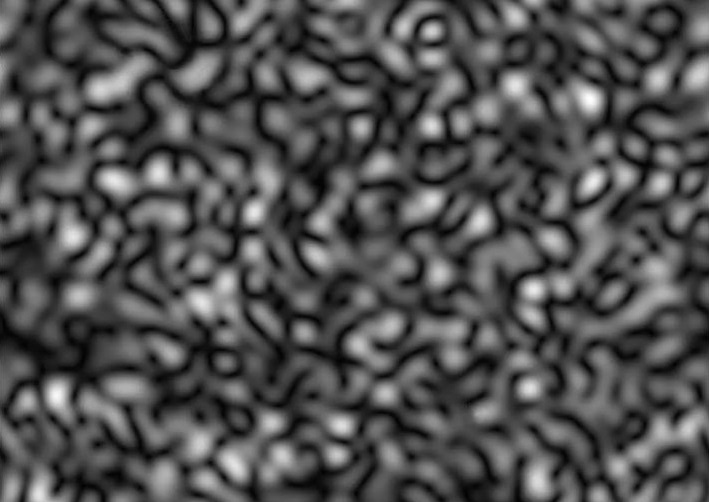
\includegraphics[frame,width=0.5\textwidth]{02_grundlagenDerDeflektometrie/rekonstruktion/stochastischeKodierung/figures/speckleMuster}
	\caption[Specklemuster]{Specklemuster.}
	\label{img:speckleMuster}
\end{figure}
%
\noindent
Das Grundprinzip der Dekodierung für dieses Kodierverfahren ist das Verfolgen der Punkte beim Verschieben des Specklemusters.
Es wird zunächst die Spiegelung des Specklemusters auf der Objektoberfläche aufgenommen und ein Referenzpunkt definiert.
Nach der Verschiebung des Specklemusters (z. B. in x-Richtung) wird dieser Referenzpunkt in dem zweiten Bild über seine Umgebung gesucht.
Dabei verwendet man einen Algorithmus zur Berechnung der zweidimensionalen Bildkorrelation, der die höchste Übereinstimmung mit der Umgebung sucht.
Wenn der verschobene Referenzpunkt gefunden wurde, wird an derselben Stelle der Punkt im ersten Bild markiert.
Der markierte Punkt ist dann der neue Referenzpunkt, der im zweiten Bild gesucht wird.
Dieser Vorgang wiederholt sich, solange die Referenzpunkte im Bild liegen.
Abbildung \ref{img:prinzipStoKodierung} zeigt schematisch das Verfahren zur Dekodierung.
%
\begin{figure}[H]
	\centering
	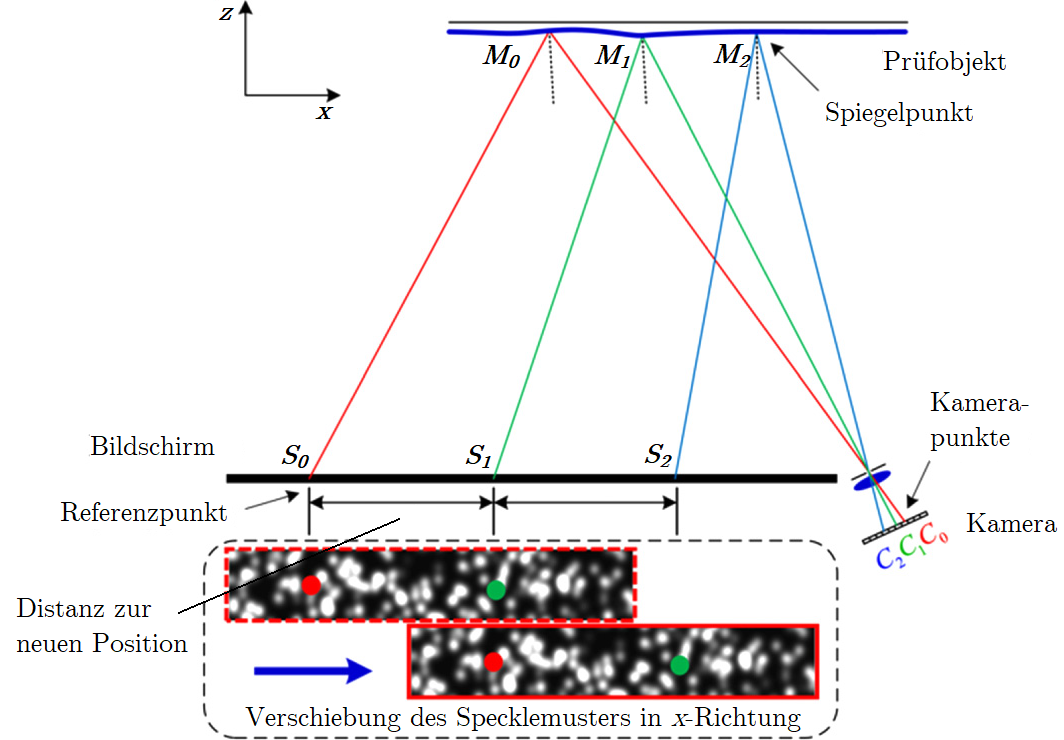
\includegraphics[width=0.9\textwidth]{02_grundlagenDerDeflektometrie/rekonstruktion/stochastischeKodierung/figures/Prinzip}
	\caption[Prinzip der Zuordnung einer stochastischen Kodierung]{Prinzip der Zuordnung einer stochastischen Kodierung. \textit{in Anlehnung an} \cite{specklePattern}}
	\label{img:prinzipStoKodierung}
\end{figure}
%
\noindent
Führt man dasselbe auch für eine andere Richtung (z. B. in y-Richtung) durch, erhält man ein Raster auf dem Objekt, an dem die Objektpunkte zugeordnet wurden (siehe Abbildung \ref{img:ergebnisStoKodierung}).
%
\begin{figure}[H]
	\centering
	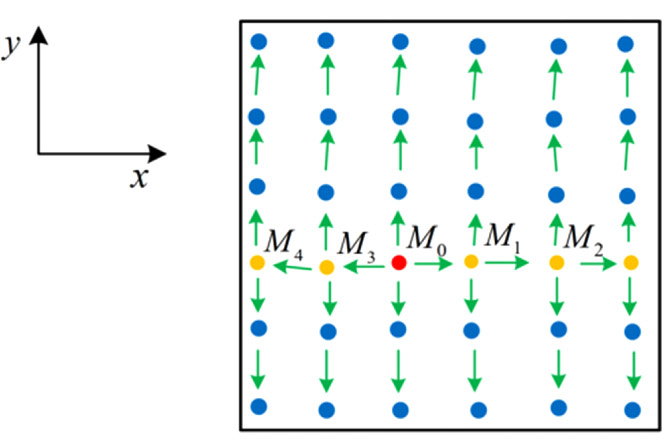
\includegraphics[width=0.4\textwidth]{02_grundlagenDerDeflektometrie/rekonstruktion/stochastischeKodierung/figures/Ergebnis}
	\caption[Ergebnis der Zuordnung einer stochastischen Kodierung]{Ergebnis der Zuordnung einer stochastischen Kodierung. Die grünen Pfeile zeigen an, von welchem Referenzpunkt man auf die nächste Zuordnung kam. \textit{in Anlehnung an} \cite{specklePattern}}
	\label{img:ergebnisStoKodierung}
\end{figure}
%
\noindent
Im Vergleich zu den vorgestellten Kodierverfahren in den vorherigen Abschnitten \ref{sub:phasenKodierung} und \ref{sub:frequenzKodierung} liefert die Dekodierung in diesem Fall nur eine begrenzte Auflösung und keine vollflächige Zuordnung.
Außerdem ist dieses Verfahren nicht anwendbar für Objekte, die eine große Verzerrung des Musters erzeugen, da die zweidimensionalen Bildkorrelation ansonsten die Referenzpunkte nicht finden kann.
Dennoch sind große Vorteile dieses Verfahrens, der geringe Rechenaufwand und die Möglichkeit, durch drei Bilder eine erfolgreiche Dekodierung durchzuführen \cite{specklePattern}.

\p
Im Rahmen der vorliegenden Arbeit wird nicht weiter auf dieses Kodierverfahren eingegangen.
}
%
% Rekonstruktion der Oberfläche und Regularisierungsproblem
{
	\FloatBarrier
    \subsection{Rekonstruktion der Oberfläche und Regularisierungsproblem}
    \label{sub:rekonstruktionUndRegularisierungsproblem}
    Durch das Vorgehen nach Abbildung \ref{tikz:abbKodierungUndDekodierung} und die beschriebenen Kodiermöglichkeiten kann die Zuordnung der Kamerapunkte und der Bildschirmpunkte erfolgen.
Mithilfe weiterer Schritte kann man daraus die Oberfläche rekonstruieren.
%
\begin{figure}[H]
	\centering
	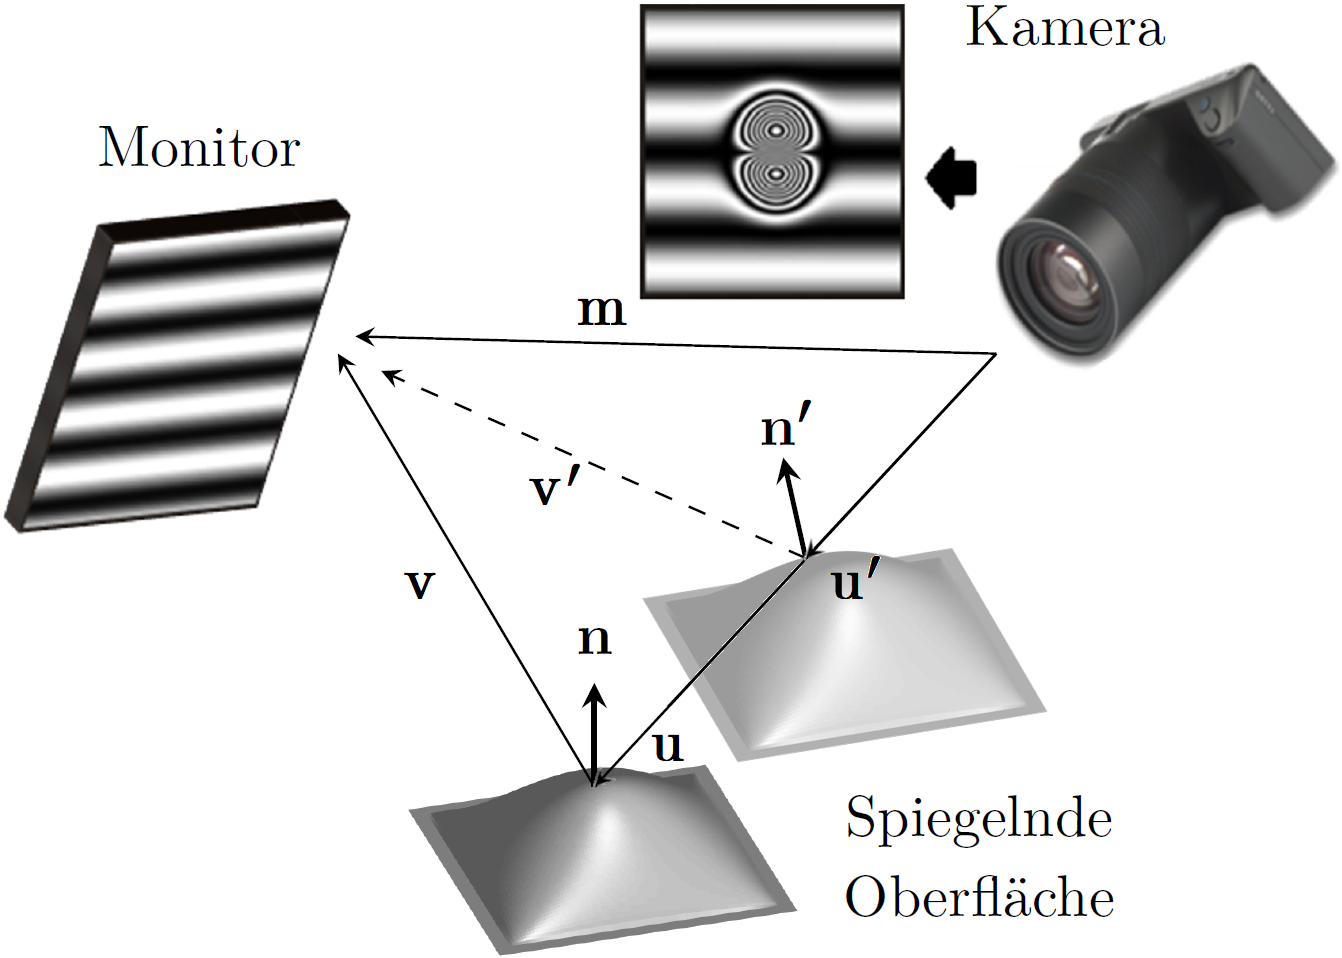
\includegraphics[width=0.7\textwidth]{02_grundlagenDerDeflektometrie/rekonstruktion/rekonstruktionUndRegularisierungsproblem/figures/regularisierungsproblem}
	\caption[Regularisierungsproblem]{Mehrere Positionsmöglichkeiten für die spiegelnde Oberfläche bei selber Zuordnung von Kamera- und Bildschirmpunkten, auch Regularisierungsproblem genannt. \textit{in Anlehnung an} \cite{stereoDeflektometrie}}
	\label{img:regularisierungsproblem}
\end{figure}
%
\noindent
Abbildung \ref{img:regularisierungsproblem} zeigt die Strahlenverfolgung zur Bestimmung der Oberflächennormalen $n$.
Zunächst benötigt man neben der Zuordnung zusätzliche Informationen über den Systemaufbau.
Das umfasst die Positionen und Ausrichtungen der Kamera und des Monitors im Raum, womit man die Zuordnung in Weltkoordinaten angeben kann.
Dadurch ist der Vektor $m$ sowie die Richtung des Sichtvektors $u$ bestimmt.
Es ist zwar bekannt, welcher Kamerapunkt durch welchen Punkt des Bildschirms beleuchtet wird, allerdings ist dadurch das optische System nicht ausreichend beschrieben, um die Länge des Sichtvektors $u$ anzugeben.
Es fehlt die Lage der Oberfläche.
Wäre diese bekannt, könnte der Reflexionsvektor $v$ mit 
\begin{equation*}
	v = m - u
\end{equation*}
bestimmt werden.
Mithilfe des Reflexionsgesetzes kann man aus dem Reflexionsvektor $v$ und dem Sichtvektor $u$ den Normalenvektor $n$ bestimmen:
%
\begin{equation}
	n = \dfrac{v - u}{\left\Vert v - u \right\Vert}
\end{equation}
%
Der Sichtvektor $u$ lässt sich für jeden Kamerapunkt aufstellen.
Berechnet man nach der Überlegung die Normalenvektoren $n$ für jeden Kamerapunkt, erhält man ein Vektorfeld, welches Normalenfeld genannt wird.
Damit wären die Neigungsinformationen der Oberfläche bekannt.

\p
Durch die unzureichende Information über die Lage der spiegelnden Oberfläche, erhält man entlang der Richtung eines Sichtvektors $u$ unendlich viele potenzielle Normalenvektoren $n'$.
Man bekommt somit auch viele verschiedene Normalenfelder für eine eindeutige Zuordnung von Kamera- und Bildschirmpunkten.
Diese Mehrdeutigkeit wird als Regularisierungs- oder Deflektometrieproblem bezeichnet.
Zur Auflösung des Regularisierungsproblems gibt es verschiedene Ansätze.
Ein solcher Ansatz ist die Stereo-Methode.
Dabei werden zwei Aufnahmen aus unterschiedlichen Positionen verwendet.
Man bestimmt für beide Aufnahmen jeweils eine Zuordnung von Kamera- und Bildschirmpunkten.
Somit entstehen für beiden Aufnahmen mehrere potenzielle Normalenfelder.
Bestimmt man die Korrelation zwischen den Normalenfeldern der unterschiedlichen Aufnahmen, sollte man eine Lage finden, an denen die Normalenfelder übereinstimmen.
Das Normalenfeld in dieser Lage entspricht damit dem tatsächlichen Normalenfeld (siehe Abbildung \ref{img:stereoVerfahren}).
Dieses und auch weitere Verfahren zur Auflösung des Regularisierungsproblems wird in der Dissertation von J. Balzer näher thematisiert\cite{regularisierungsproblem}.
%
\begin{figure}[H]
	\centering
	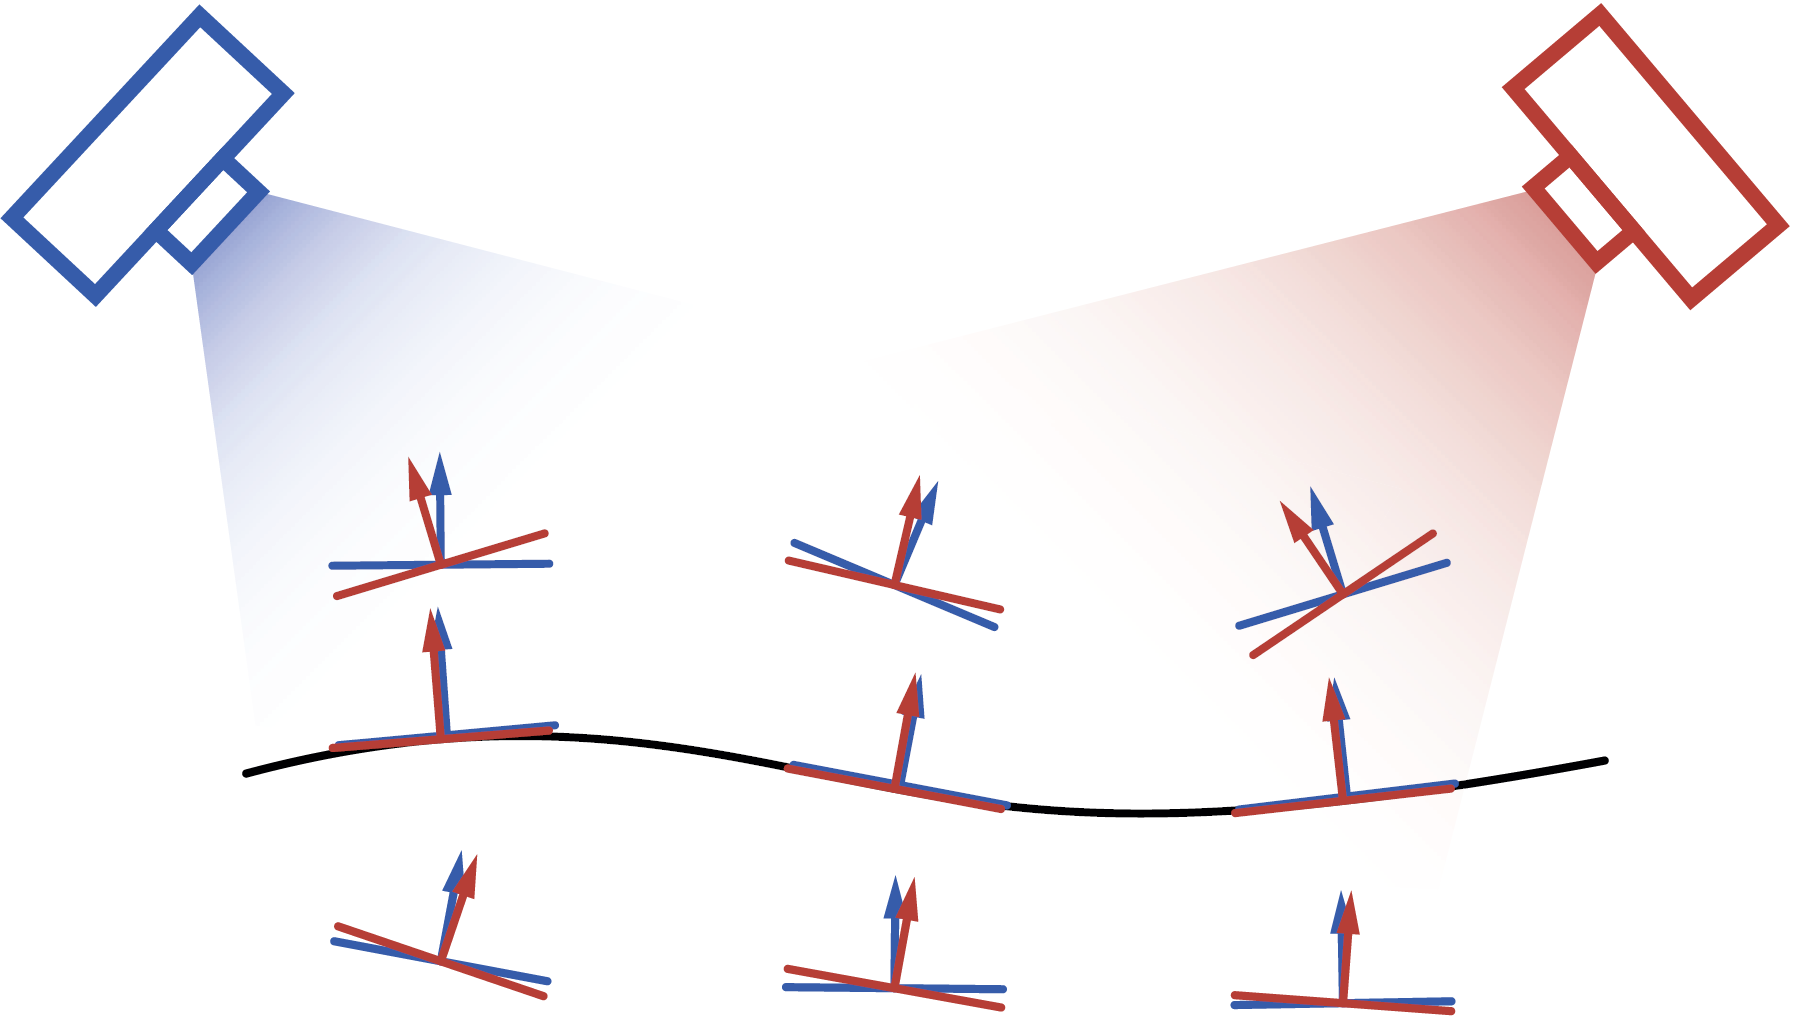
\includegraphics[width=0.5\textwidth]{02_grundlagenDerDeflektometrie/rekonstruktion/rekonstruktionUndRegularisierungsproblem/figures/stereoVerfahren}
	\caption[Stereo-Methode zur Lösung des Regularisierungsproblems]{Stereo-Methode zur Auflösung der Mehrdeutigkeit der Normalenfelder. Die eingezeichneten Pfeile sind die potentiellen Normalenvektoren auf unterschiedlichen Höhen. \cite{stereoDeflektometrie}}
	\label{img:stereoVerfahren}
\end{figure}
%
\noindent
Schließlich ist es möglich, aus dem Normalenfeld die räumlichen Informationen der Oberfläche zu berechnen.
Dafür kann man zunächst aus den Normalenvektoren die zugehörigen Tangentialebenen berechnen, die über je zwei Richtungsvektoren definiert sind.
Diese Richtungsvektoren bilden die Tangentialfelder des Prüfobjekts.
Man kann über eine Integration der Tangentialfelder in ausgewählte Richtungen Kurven bestimmen, die auf der Oberfläche des Objekts liegen.
Durch diese Integration erhält man einen Höhenzusammen\-hang der Oberflächenpunkte.
Wenn zusätzlich die Lage eines Oberflächenpunkts im Raum gegeben ist, kann man die Positionen der Oberflächenpunkte im Raum angeben \cite{kit_werling}.
}
%

}

%Qualitative Sichtprüfung
{
	\FloatBarrier
    \section{Qualitative Sichtprüfung}
    \label{sec:qualitativeSichtpruefung}
    Der Bereich der qualitativen Sichtprüfung hat grundlegend die Aufgabe, spiegelnde Oberflächen nach bestimmten Kriterien in gut und fehlerhaft zu unterteilen.
Die Aufbauten für solche Verfahren sehen in der Regel ähnlich aus wie auch in Abbildung \ref{img:aufbau}.
Zur Analyse dieser spiegelnden Oberflächen ist es nicht unbedingt nötig, zuerst ein dreidimensionales Oberflächenmodell zu erzeugen.
Ein wesentlicher Unterschied ist deshalb, dass die Informationen über den Systemaufbau nicht zwingend notwendig für Berechnungen sind.
Um eine möglichst allgemein einsetzbare Lösung zu entwickeln, ist dies ein essenzieller Vorteil.
Die Vorgehensweise bei diesen Verfahren basiert in den meisten Fällen darauf, die Abweichungen der Oberflächenstruktur zu einem Referenzobjekt zu bewerten.
Abhängig von den einzelnen Oberflächenmerkmalen können verschiedene Muster und Strategien zur Auswertung eingesetzt werden.

\p
In seiner Dissertation \glqq Deflektometrie zur automatischen Sichtprüfung und Rekonstruktion spiegelnder Oberflächen\grqq ~\cite{kit_werling} listet Stefan Bruno Werling vom Karlsruher Institut für Technologie einige Auswertungsmöglichkeiten auf.
Daraus sind die Folgenden eine Auswahl seiner Strategien:

\begin{itemize}
	\item Untersucht man auf der Oberfläche eines Objekts ein sinusoidales Streifenmuster, dann können im Frequenzraum Abweichungen des Musters von einem \glqq Idealmuster\grqq ~bzw. Referenzmuster festgestellt werden.
	Dadurch entdeckt man Unterschiede in der Oberflächenkrüm\-mung.
	Die Transformation des Bildes in den Frequenzraum wird durch die Fourier-Transformation erreicht.
	
	\item Nutzt man zur Auswertung ein Schachbrettmuster, so können durch die Wahl eines geeigneten Schwellwerts bestimmte Flächen segmentiert und geometrisch analysiert werden.
	Nach der Analyse sollen Anomalien der geometrischen Merkmale Aussagen über die Krümmung treffen.
	
	\item Besonders kleine Fehler und Defekte der Oberflächenstruktur lassen sich an Hell-Dunkelübergängen gut hervorheben.
	Hierfür kann man einfache Streifenmuster analysieren, wie es in Abbildung \ref{img:scratch} gezeigt ist.
	Dieses Verfahren wird im Kapitel \ref{chp:sichtpruefungDurchLichtstreuung} näher beschrieben.
\end{itemize}

\begin{figure}[H]
	\centering
	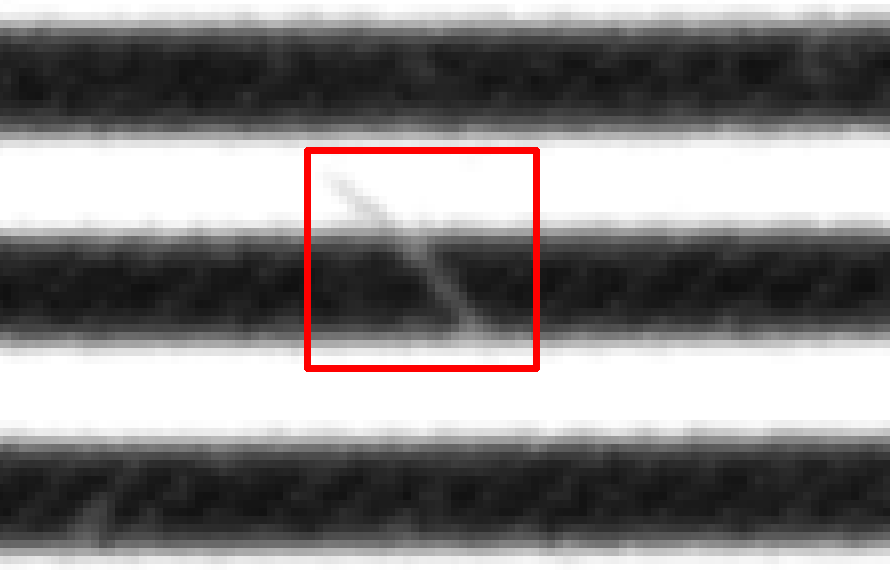
\includegraphics[width=0.5\textwidth]{02_grundlagenDerDeflektometrie/qualitativeSichtpruefung/figures/scratch}
	\caption[Kratzer an Hell-Dunkel-Übergang eines Streifenmusters]{Kratzer an Hell-Dunkel-Übergang eines Streifenmusters}
	\label{img:scratch}
\end{figure}

\noindent
Neben diesen Verfahren gibt es auch noch die Möglichkeit, die Krümmung zu analysieren, indem man die Zuordnung zwischen Kamera- und Bildschirmkoordinaten (siehe Abschnitt \ref{sec:rekonstruktion}) auswertet.
Analytisch betrachtet ändert sich bei starken lokalen Krümmungen der Oberfläche auch die Oberflächennormale an der lokalen Stelle besonders stark.
Mit dem Reflexionsgesetz wird damit kenntlich, dass lokal in der Reflexion große Abweichungen von einer ebenen Spiegelung auftreten.
Die Abweichung von einer ebenen Spiegelung lässt sich in der beschriebenen Zuordnung direkt erkennen, ohne weitere Systemparameter berücksichtigen zu müssen.
Dies wird im Abschnitt \ref{sec:auswertungDeflektometrischeRegistrierung} genauer behandelt.

\p
Durch die Variabilität der deflektometrische Verfahren und der vielen Möglichkeiten der qualitativen Sichtprüfung lassen sich z. B. durch Veränderung bestimmter Muster zahlreiche verschiedene Verfahren aufstellen, um eine Objektoberfläche zu analysieren.
Aus dem Grund wird keine allgemeine Funktionsweise von deflektometrischen Verfahren für die qualitative Sichtprüfung beschrieben, sondern auf konkrete Verfahren eingegangen, wie es z. B. in Kapitel \ref{chp:sichtpruefungDurchLichtstreuung} ausgeführt wird.
}
	}
	
	%Sichtprüfung durch Lichtstreuung
	{
		\FloatBarrier %Verhindert Fehlpositionierung von Abbildungen aus vorherigen Abschnitten
		\chapter{Sichtprüfung durch Lichtstreuung}
		\label{chp:sichtpruefungDurchLichtstreuung}
		Dieses Kapitel legt den Schwerpunkt auf die Erkennung von kleinen Oberflächendefekten auf transparenten Prüfobjekten.
Darunter sollen insbesondere Kratzer auf Brillengläsern kenntlich gemacht werden.

%Prüfaufbau
{
	\FloatBarrier
    \section{Prüfaufbau}
    \label{sec:pruefaufbau}
    Die folgende Abbildung \ref{img:pruefaufbau} zeigt eine Skizze des verwendeten Prüfaufbaus.
Zur Vereinfachung werden in der Skizze keine Halterungen dargestellt.

\begin{figure}[H]
	\centering
	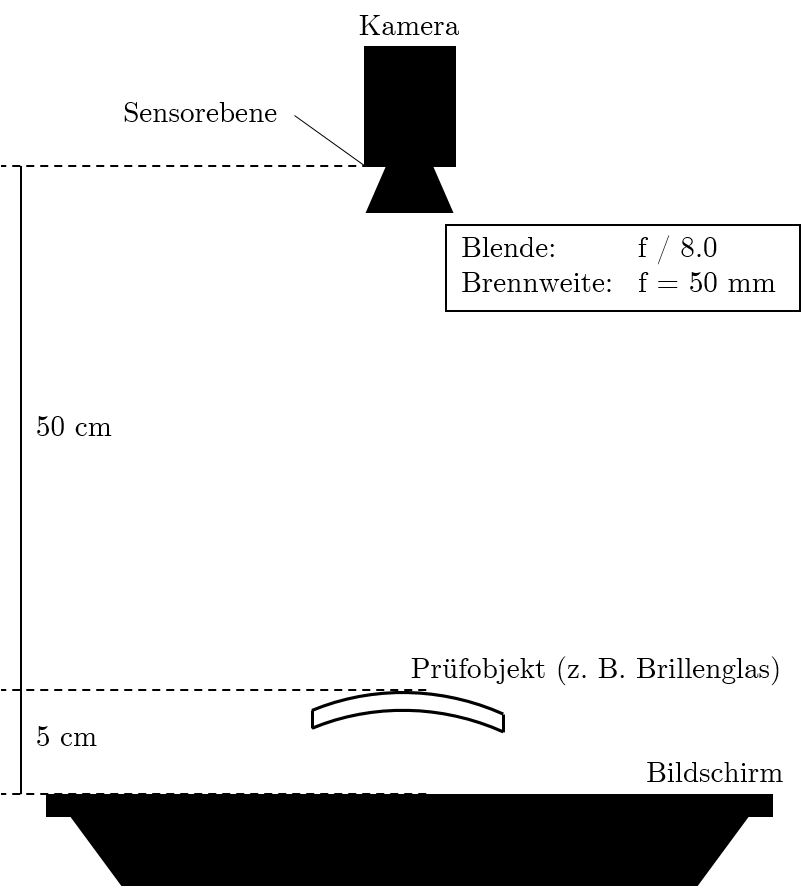
\includegraphics[width=0.5\textwidth]{03_sichtpruefungDurchLichtstreuung/pruefaufbau/figures/aufbau}
	\caption[Prüfaufbau]{Prüfaufbau (Abbildung nicht maßstabsgetreu)}
	\label{img:pruefaufbau}
\end{figure}

\noindent
Die Parameter des Prüfaufbaus wie z. B. Kameraeinstellungen und Entfernungen lassen sich aus Abbildung \ref{img:pruefaufbau} entnehmen.
Es gilt zu beachten, dass die Entfernung der Prüfobjekte zur Kamera nicht am Objektiv, sondern an der Sensorebene gemessen wird.
Der Grund liegt darin, dass Objektive unterschiedliche Größen haben, weshalb die Entfernung für verschiedene Objektive unterschiedlich sein würde.
Die Sensorebene einer Kamera ist die Position des Kamerasensors, an der das einfallende Licht aufgenommen wird.
Zur Erzeugung des Bildmaterials wird ein Monitor als Durchlichtbeleuchtung verwendet, um die speziellen Eigenschaften der Lichtstreuung an den Oberflächenbeschädigungen zu nutzen.
Auf diese Eigenschaften wird im Kapitel \ref{sec:verfahren} weiter eingegangen.
Die Objekte zwischen der Kamera und der Beleuchtung sind dabei transparente Brillengläser mit Oberflächenbeschädigungen.
Die Oberflächenbeschädigungen umfassen Eingravierungen, Kratzer und ähnliche Fehlstellen.
}

%Verfahren
{
	\FloatBarrier
    \section{Verfahren}
    \label{sec:verfahren}
    Es soll ein Verfahren beschrieben werden, dass es ermöglicht, Kratzer und ähnliche Defekte mittels Methoden aus der Deflektometrie sichtbar zu machen.
Man nutzt die abweichende Lichtstreuung an Kratzern und anderen Oberflächenbeschädigungen im Gegensatz zur idealen Oberfläche des Objekts.
Das beschriebene Verfahren lässt sich mit geeigneter Anpassung des Versuchsaufbaus auch auf spiegelnde Oberflächen anwenden.
Dabei gilt zu beachten, dass Spiegelbilder anstelle von Bildern der Durchlichtprojektionen ausgewertet werden.

\begin{figure}[H]
	\centering
	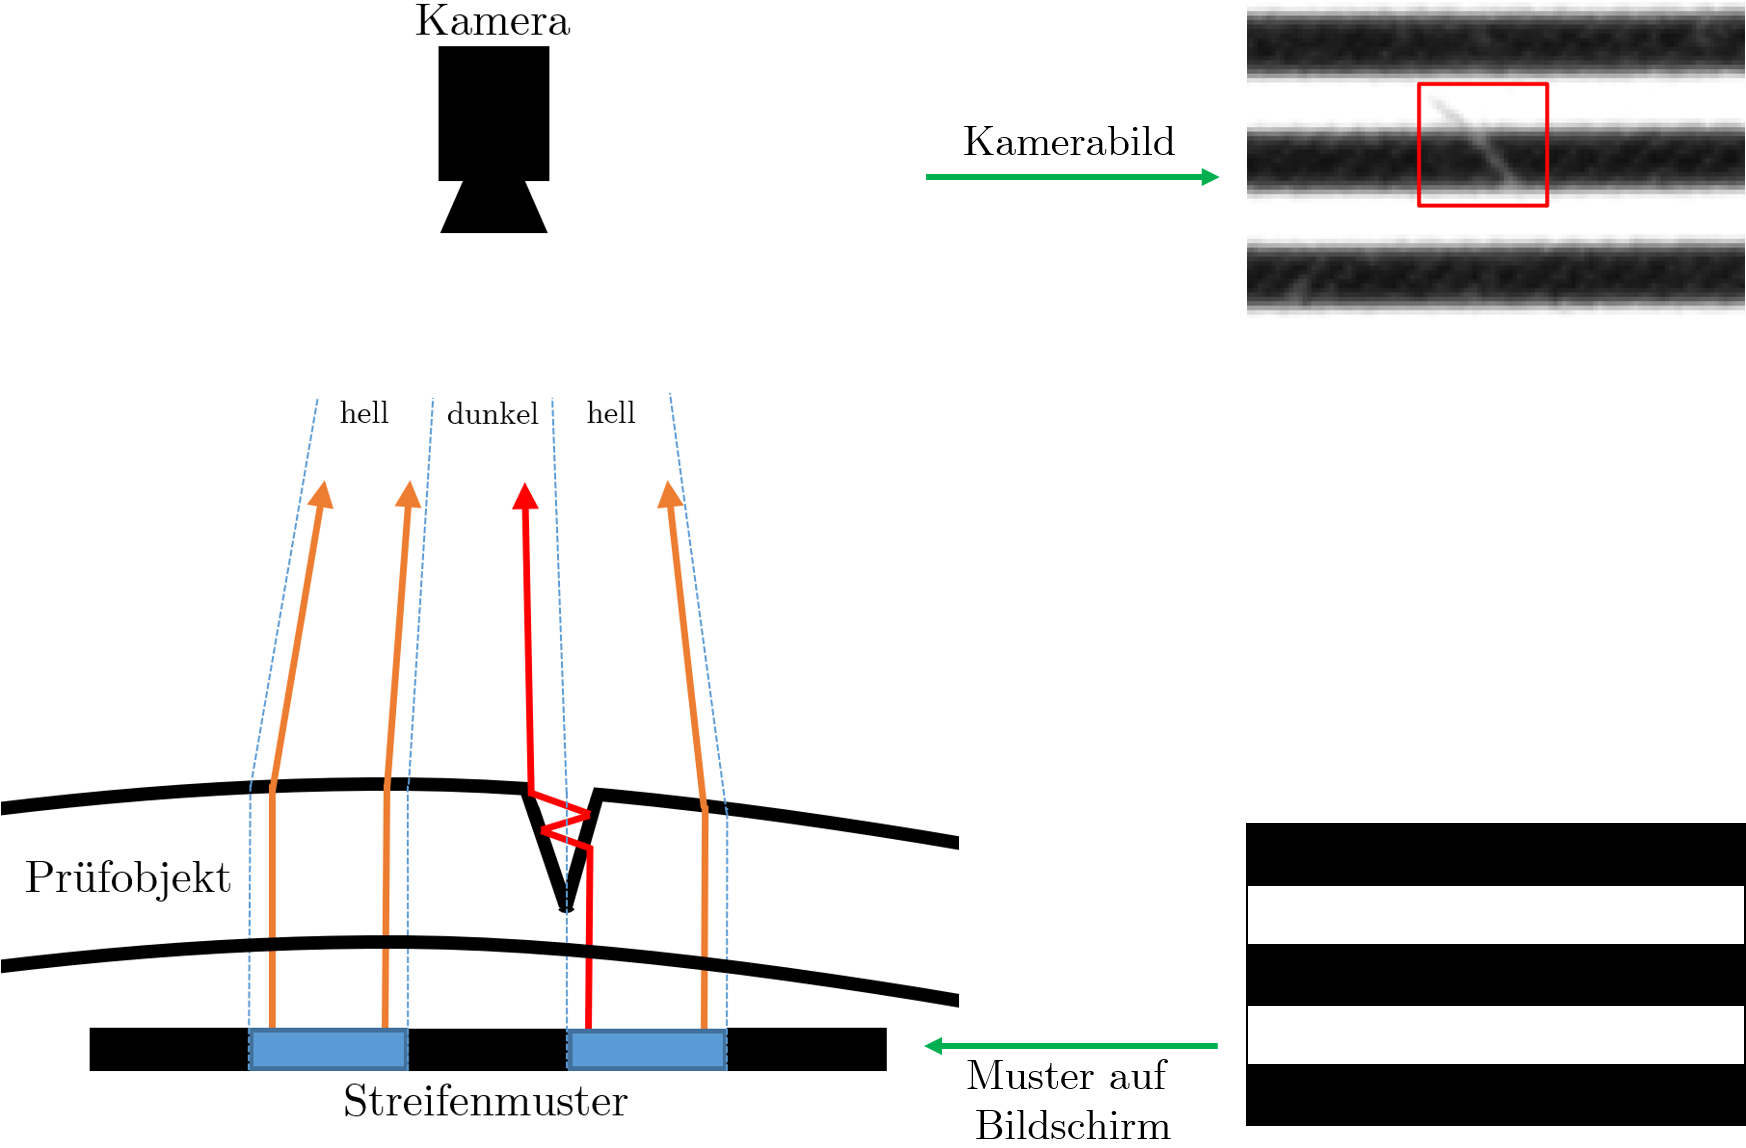
\includegraphics[width=\textwidth]{03_sichtpruefungDurchLichtstreuung/verfahren/figures/scratch_reflection_with_images}
	\caption[Lichtbrechung an einem Kratzer]{Querschnitt eines Brillenglases mit Lichtbrechung an einem Kratzer. Die blauen Stellen entsprechen den hellen Streifen und die schwarzen Stellen den dunklen Streifen auf dem Monitor. (Abbildung nicht maßstabsgetreu)}
	\label{img:lightreflection}
\end{figure}

\noindent
In Abbildung \ref{img:lightreflection} wird schematisch die Überlegung hinter dem Ansatz dargestellt.
Man nimmt ein Streifenmuster und projiziert dieses auf ein spiegelndes Prüfobjekt.
Für ein transparentes Prüfobjekt kann man das Streifenmuster als Durchlichtbeleuchtung von unten projizieren.
Mit der Kamera wird schließlich eben dieses projizierte Muster aufgenommen.
Dabei fällt an den Hell-Dunkelübergängen Licht vom hellen Streifen in den Kratzer.
Durch den Kratzer werden manche Lichtstrahlen so gestreut, dass diese an der Stelle des dunklen Streifens in den Kamerasensor gelangen (siehe roten Lichtstrahl in Abbildung \ref{img:lightreflection}).
Man erkennt im Kamerabild eine lokale Fehlstelle, da der Kratzer heller ist als der umliegende dunkle Streifen.
Analog dazu erkennt man im hellen Streifen lokal eine etwas dunklere Stelle.
Durch Anpassung der Kameraeinstellungen kann man beeinflussen, wie deutlich man den Kratzer sieht.
Z. B. kann dies durch die Erhöhung der Belichtungszeit oder weitere Öffnung der Blende geschehen.
Dadurch wird ein Oberflächendefekt im dunklen Streifen zwar besser und stärker sichtbar, allerdings ist es möglich, die Informationen über den Defekt im hellen Streifen zu verlieren.
Dies liegt daran, dass auch die dunklere Stelle im hellen Streifen so hell werden kann, dass sie nicht mehr von dem hellen Streifen selbst zu unterscheiden ist.
Dieses Problem erkennt man in der Abbildung \ref{img:scratches}.

\begin{figure}[H]
	\centering
	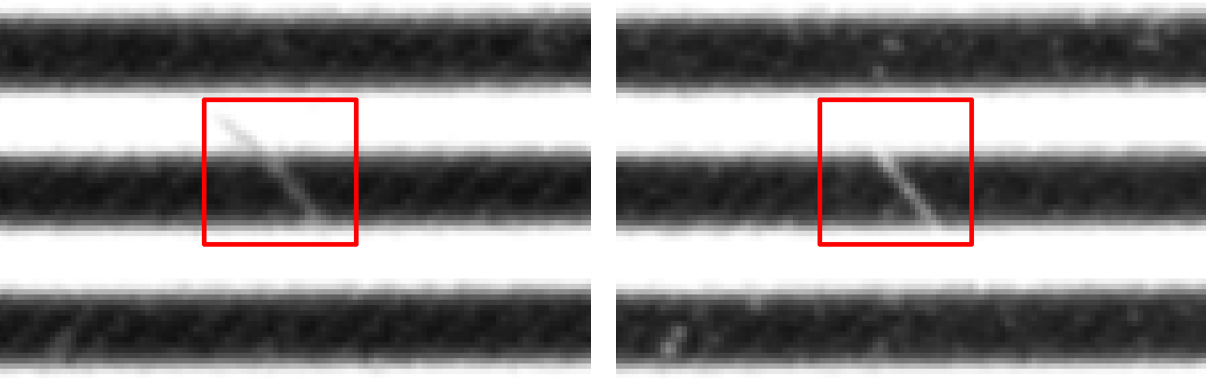
\includegraphics[width=\textwidth]{03_sichtpruefungDurchLichtstreuung/verfahren/figures/visibleScratch}
	\caption[Kratzer]{Kratzer an Hell-Dunkel-Übergang. Links mit weniger weit geöffneten Blende im Vergleich zu rechts.}
	\label{img:scratches}
\end{figure}

\noindent
Trotz der fehlenden Information hat das rechte Bild den Vorteil, dass durch den höheren Kontrast zwischen dem Oberflächendefekt und dem Hintergrund eine bessere Erkennung möglich ist.
Je ausgeprägter die Beschädigung in der Oberfläche ist, desto mehr Licht wird an der Stelle gestreut und die Beschädigung wird besser erkennbar.

\begin{figure}[H]
	\centering
	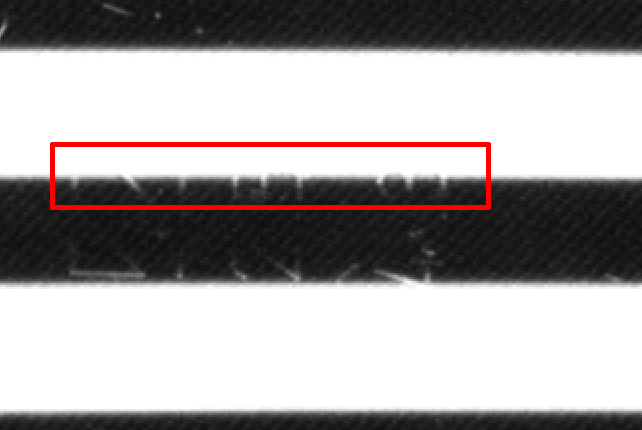
\includegraphics[width=\textwidth]{03_sichtpruefungDurchLichtstreuung/verfahren/figures/minorScratch}
	\caption[Eingravierung im Glas]{Schlecht erkennbare Eingravierung im Glas, nach Verschiebung des Streifenmusters.}
	\label{img:engraving}
\end{figure}

\noindent
In Abbildung \ref{img:engraving} stellt man fest, dass kleine Defekte der Oberflächenstruktur, wie hier z. B. die Eingravierung, nur zum Teil und besonders in der Nähe der Übergänge zu erkennen sind.

\p
Daraus lassen sich bestimmte Folgerungen ziehen.
Zunächst decken solche Streifenmuster nur unmittelbar an den Übergängen zuverlässig Defekte auf.
Das bedeutet, um Defekte an bestimmten Stellen zu erfassen, muss das verwendete Streifenmuster an den Stellen Übergänge haben.
Das bedeutet auch, dass Muster mit schmaleren Streifen aufgrund weiterer Übergänge besser geeignet sind, um auch kleinere Oberflächendefekte sichtbar zu machen.
Allerdings führt dies auch dazu, dass stets nur kleine Teile der Defekte zu erkennen sind.
Als Lösung dieses Problems kann man mehrere Streifenmuster verwenden, deren Streifen stets in ihrer Ausbreitungsrichtung verschoben sind.
Verknüpft man die sichtbaren Teile der Defekte, kann man in einem vollständigen Gesamtbild alle Oberflächendefekte ab einer bestimmten Mindeststärke sichtbar machen.
Die Mindeststärke hängt dabei unter anderem von den Kameraeinstellungen, der Beleuchtungsstärke und den verwendeten Streifenmustern ab.
}

%Einsatz von mehreren Streifenmustern
{
	\FloatBarrier
    \section{Einsatz von mehreren Streifenmustern}
    \label{sec:einsatzVonMehrerenStreifenmustern}
    Die verwendeten Streifenmuster haben entlang ihrer Ausbreitungsrichtung den Grauwerteverlauf einer Rechteckschwingung.

\noindent
Die periodische Einheitsrechteckschwingung $s_f(t)$ sei definiert durch (vgl. \cite{squareWave}):
%
\begin{equation} \label{eq:einheitsrechteckschwingung}
	s_f(t) := \sign \left( \sin \left(2 \pi f t \right) \right)
\end{equation}
%
$\sign(x)$ bezeichnet hierbei die Vorzeichenfunktion mit:
%
\begin{equation*}
	\sign(x) := 
		\begin{cases}
	      -1 & \text{für $x < 0$}\\
	      0 & \text{für $x = 0$}\\
	      1 & \text{für $x > 0$}
	    \end{cases} 
\end{equation*}
%
Die Periodendauer $T$ der Einheitsrechteckschwingung $s_f(t)$ steht über den Kehrwert im Zusammenhang mit der Frequenz $f$:
\begin{equation*}
	T = \dfrac{1}{f}
\end{equation*}
Für $f = \tfrac{1}{3}$ und $f = \tfrac{1}{4}$ sieht das Schaubild der Funktion aus wie in Abbildung \ref{tikz:abbRechteckschwingung}:
% Abbildung: Rechteckschwingung
{
	\begin{figure}[H]
		\centering
		\begin{adjustbox}{width=\textwidth}
	\begin{tikzpicture}
	
		% Koordinatensystem 1
		\draw[thick,-stealth,black] (-8,0)--(8,0) node[below] {$t$};
		\draw[thick,-stealth,black] (0,-2.125)--(0,2.125) node[left] {$s_{\tfrac{1}{3}}(t)$};
		
		% Funktion 1
		\draw[name path = func1, blue, thick, domain=-8:8, samples=600] plot (\x,{1.5*(sign(sin(2*pi*(1/3)*\x r))});

		% Achsenbeschriftungen 1
		\draw[thick,black] (0,-1.5) -- (-0.1,-1.5) node[anchor=east,fill=white] {$-1$};
		\draw[thick,black] (0,1.5) -- (-0.1,1.5) node[anchor=east,fill=white] {$1$};
		\draw[thick,black] (-7,0) -- (-7,-0.1) node[anchor=north,fill=white] {$-7$};
		\draw[thick,black] (-6,0) -- (-6,-0.1) node[anchor=north,fill=white] {$-6$};
		\draw[thick,black] (-5,0) -- (-5,-0.1) node[anchor=north,fill=white] {$-5$};
		\draw[thick,black] (-4,0) -- (-4,-0.1) node[anchor=north,fill=white] {$-4$};
		\draw[thick,black] (-3,0) -- (-3,-0.1) node[anchor=north,fill=white] {$-3$};
		\draw[thick,black] (-2,0) -- (-2,-0.1) node[anchor=north,fill=white] {$-2$};
		\draw[thick,black] (-1,0) -- (-1,-0.1) node[anchor=north,fill=white] {$-1$};
		\draw[thick,black] (1,0) -- (1,-0.1) node[anchor=north,fill=white] {$1$};
		\draw[thick,black] (2,0) -- (2,-0.1) node[anchor=north,fill=white] {$2$};
		\draw[thick,black] (3,0) -- (3,-0.1) node[anchor=north,fill=white] {$3$};
		\draw[thick,black] (4,0) -- (4,-0.1) node[anchor=north,fill=white] {$4$};
		\draw[thick,black] (5,0) -- (5,-0.1) node[anchor=north,fill=white] {$5$};
		\draw[thick,black] (6,0) -- (6,-0.1) node[anchor=north,fill=white] {$6$};
		\draw[thick,black] (7,0) -- (7,-0.1) node[anchor=north,fill=white] {$7$};
		
		% Beschriftung für f
		\draw[blue,thick] node[anchor=west] at (-8,2.125) {$f = \tfrac{1}{3}$:};
		
		
		% Koordinatensystem 2
		\draw[thick,-stealth,black] (-8,-5)--(8,-5) node[below] {$t$};
		\draw[thick,-stealth,black] (0,-7.125)--(0,-2.875) node[left] {$s_{\tfrac{1}{4}}(t)$};
				
		% Funktion 2
		\draw[name path = func2, Green, thick, domain=-8:8, samples=600] plot (\x,{(1.5*(sign(sin(2*pi*(1/4)*\x r)))-5});
				
		% Achsenbeschriftungen 2
		\draw[thick,black] (0,-6.5) -- (-0.1,-6.5) node[anchor=east,fill=white] {$-1$};
		\draw[thick,black] (0,-3.5) -- (-0.1,-3.5) node[anchor=east,fill=white] {$1$};
		\draw[thick,black] (-7,-5) -- (-7,-5.1) node[anchor=north,fill=white] {$-7$};
		\draw[thick,black] (-6,-5) -- (-6,-5.1) node[anchor=north,fill=white] {$-6$};
		\draw[thick,black] (-5,-5) -- (-5,-5.1) node[anchor=north,fill=white] {$-5$};
		\draw[thick,black] (-4,-5) -- (-4,-5.1) node[anchor=north,fill=white] {$-4$};
		\draw[thick,black] (-3,-5) -- (-3,-5.1) node[anchor=north,fill=white] {$-3$};
		\draw[thick,black] (-2,-5) -- (-2,-5.1) node[anchor=north,fill=white] {$-2$};
		\draw[thick,black] (-1,-5) -- (-1,-5.1) node[anchor=north,fill=white] {$-1$};
		\draw[thick,black] (1,-5) -- (1,-5.1) node[anchor=north,fill=white] {$1$};
		\draw[thick,black] (2,-5) -- (2,-5.1) node[anchor=north,fill=white] {$2$};
		\draw[thick,black] (3,-5) -- (3,-5.1) node[anchor=north,fill=white] {$3$};
		\draw[thick,black] (4,-5) -- (4,-5.1) node[anchor=north,fill=white] {$4$};
		\draw[thick,black] (5,-5) -- (5,-5.1) node[anchor=north,fill=white] {$5$};
		\draw[thick,black] (6,-5) -- (6,-5.1) node[anchor=north,fill=white] {$6$};
		\draw[thick,black] (7,-5) -- (7,-5.1) node[anchor=north,fill=white] {$7$};
		
		% Beschriftung für f
		\draw[Green,thick] node[anchor=west] at (-8,-2.875) {$f = \tfrac{1}{4}$:};
		
	\end{tikzpicture}
\end{adjustbox}
\caption[Rechteckschwingung bzw. \textit{engl.: square wave}]{Einheits-Rechteckschwingung (\textit{engl.: square wave}) für $f = \tfrac{1}{3}$ (in blau) und $f = \tfrac{1}{4}$ (in grün).}
		\label{tikz:abbRechteckschwingung}
	\end{figure}
}

\noindent
Mithilfe der Einheitsrechteckschwingung aus Gleichung \ref{eq:einheitsrechteckschwingung} lässt sich ein Streifenmuster mit Ausbreitungsrichtung in $x$ ausdrücken durch:
\begin{equation} \label{eq:rstreifenmuster}
	\begin{gathered}
		m_k(x,y) = A_m 
		\left(
			1 + s_f \left(x - \dfrac{1}{2\pi f} \psi_k \right)
		\right),\\
		f = \dfrac{N_p}{\acrshortmath{lwidth}},
		\quad
		\psi_k = (k - 1)\dfrac{2\pi}{N_{shift}},
		\quad
		k \in \lbrace 1,\ldots,N_{shift}\rbrace 
	\end{gathered}
\end{equation}
%
Das Streifenmuster aus Gleichung \ref{eq:rstreifenmuster} ist durch die Periodizität der Einheitsrechteckschwingung auch periodisch zur Ausbreitungsrichtung.
$A_m$ bezeichnet die Amplitude, $f$ die Frequenz, $N_p$ die Anzahl der Perioden über die Monitorbreite \acrshort{lwidth}, $N_{shift}$ die Anzahl der Phasenverschiebungen und $\psi_k$ die Phasenverschiebung des $k$-ten Musters.
Analog zu Gleichung \ref{eq:rstreifenmuster} lassen sich auch Streifenmuster mit Ausbreitungsrichtung in $y$ über die Monitorhöhe \acrshort{lheight} beschreiben.
Das Bild eines vertikalen Streifenmusters, d. h. mit Ausbreitungsrichtung in $x$, nach Gleichung \ref{eq:rstreifenmuster} wird in Abbildung \ref{tikz:abbRechteckStreifenmuster} dargestellt.

% Abbildung: Rechteck Streifenmuster
{
	\begin{figure}[H]
		\centering
		\begin{adjustbox}{width=\textwidth}
	\begin{tikzpicture}[every node/.style={inner sep=0,outer sep=0}]
	
		\node [anchor=north east] (img1) at (-0.03\textwidth,0) {
\includegraphics[frame,width=.47\textwidth]{03_sichtpruefungDurchLichtstreuung/einsatzVonMehrerenStreifenmustern/figures/rechteckStreifenmuster}};
		\node [below=0.2cm of img1] {Muster $m_1$ mit $\psi_1 = 0$};
		\node [anchor=north west] (img2) at (0.03\textwidth,0) {
\includegraphics[frame,width=.47\textwidth]{03_sichtpruefungDurchLichtstreuung/einsatzVonMehrerenStreifenmustern/figures/rechteckStreifenmuster_shifted}};
		\node [below=0.2cm of img2] {Muster $m_2$ mit $\psi_2 = \tfrac{\pi}{2}$};
		
	\end{tikzpicture}
\end{adjustbox}
\caption[Rechteckförmiges Streifenmuster]{Streifenmuster nach Gleichung \ref{eq:rstreifenmuster}, mit $A_m = 127.5$, $N_p = 6$, $N_{shift} = 4$ und $\acrshortmath{lwidth} = 384$. Die Breite der Streifen betragen jeweils 32 Pixel.}
		\label{tikz:abbRechteckStreifenmuster}
	\end{figure}
}
%
\noindent
Die verschiedenen Streifenmuster $m_k$ können nach Gleichung \ref{eq:rstreifenmuster} als zueinander phasenverschoben bezeichnet werden.
Die Phasenverschiebung $\psi_k$ wird durch einen Phasenwinkel im Bogenmaß angegeben.
Eine Phasenverschiebung von $ \pi $ bedeutet dementsprechend eine Phasenverschiebung um eine halbe Periode des Musters.
Anschaulich stellt man fest, dass für gleich breite helle und dunkle Streifen diese ihre Positionen tauschen.
Dies kann man sich zunutze machen, denn das bedeutet, dass die Schnittmenge der dunklen Streifen in den beiden Streifenmustern am kleinsten ist.
Da bestimmte Fehlstellen entweder in den dunklen oder in den weißen Streifen deutlich zu erkennen sind, ergänzen sich die beiden Streifenmuster durch die sichtbaren Fehlstellen.
Verknüpft man die Kamerabilder von solchen Mustern, dann kann man damit die meiste Information aus zwei Bildern extrahieren.
Durch zusätzliche Bildaufnahmen mit verschobenen Streifenmustern kann man detailliertere Oberflächeninformationen von dem Prüfobjekt gewinnen.

\begin{figure}[H]
	\centering
	
\includegraphics[width=\textwidth]{03_sichtpruefungDurchLichtstreuung/einsatzVonMehrerenStreifenmustern/figures/imageToLink}
	\caption[Zu verknüpfende Bilder]{Kameraaufnahme eines Prüfobjekts unter Beleuchtung durch Streifenmustern mit einer Phasenverschiebung von $ \pi $ zueinander.}
	\label{img:imageToLink}
\end{figure}

\noindent
Wie man erkennt, sind die Streifen der beiden Bilder genau zueinander versetzt.
Die Auffälligkeiten in den Bildern wie z. B. Eingravierungen sind oft entweder in den dunklen oder in den hellen Streifen zu erkennen.
Durch den Unterschied zum Streifenhintergrund erfasst man gewisse Oberflächeninformationen des Prüfobjekts.
Das heißt, dass die beiden Bilder sich durch den Versatz in ihrer Oberflächeninformation ergänzen.
Zur Verknüpfung der Informationen in einem Gesamtbild überlegt man sich, wie bestimmte Defekte in den beiden Bildern aussehen.
Die Defekt- und Fehlstellen werden in zwei Fälle unterteilt (siehe Abbildung \ref{img:imageToLinkWithMarkings}).

\begin{figure}[H]
	\centering
	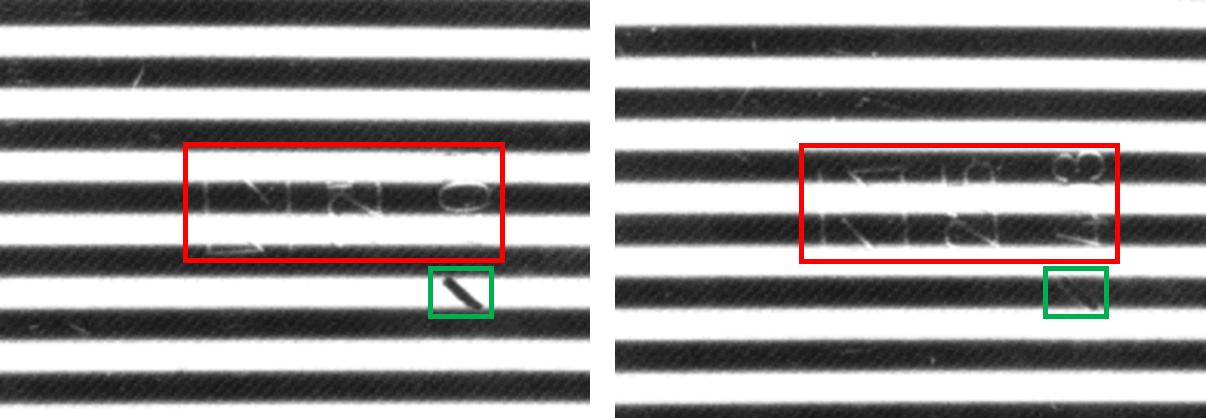
\includegraphics[width=\textwidth]{03_sichtpruefungDurchLichtstreuung/einsatzVonMehrerenStreifenmustern/figures/imageToLinkWithMarkings}
	\caption[Markierte Fehlstellen]{Kameraaufnahme eines Prüfobjekts mit Fehlstellen und deren Kennzeichnung. Im linken Teilbild Aufnahme des Musters $m_1$. Im rechten Teilbild Aufnahme des Musters $m_2$.}
	\label{img:imageToLinkWithMarkings}
\end{figure}

\noindent
\textbf{Fall 1: z. B. Kratzer (siehe rote Rechtecke in Abbildung \ref{img:imageToLinkWithMarkings})}
\nopagebreak
\par\medskip\noindent
\begin{tabular}{@{} p{0.438888889\textwidth} c p{0.438888889\textwidth} @{}}
	Aufnahme von Muster $m_1$ &  & Aufnahme von Muster $m_2$ \\ 
	Helle Fragmente in dunklen Streifen & $ \longleftrightarrow $ & Helle Fragmente in hellen Streifen \\ 
\end{tabular}

\p
\textbf{Fall 2: z. B. Partikel (siehe grüne Rechtecke in Abbildung \ref{img:imageToLinkWithMarkings})}
\nopagebreak
\par\medskip\noindent
\begin{tabular}{@{} p{0.438888889\textwidth} c p{0.438888889\textwidth} @{}}
	Aufnahme von Muster $m_1$ &  & Aufnahme von Muster $m_2$ \\ 
	Dunkle Fragmente in hellen Streifen & $ \longleftrightarrow $ & Dunkle Fragmente in dunklen Streifen \\ 
\end{tabular}

\p
Die Muster $m_1$ und $m_2$ sind Streifenmuster, die zueinander um $ \pi $ phasenverschoben sind.
Für eine Verknüpfung von Bildern errechnet man ein neues Bild, indem man zwei Bilder punktweise zusammen verrechnet.
Das bedeutet, um für das Ergebnisbild den Grauwert an der Stelle $ (x,y) $ zu berechnen, verknüpft man die beiden Grauwerte der Eingangsbilder an der gleichen Stelle $ (x,y) $.
Daraus folgt auch, dass die zu verrechnenden Bilder dieselbe Größe haben müssen.
Diese Bedingung ist hier durch dieselben Kameraeinstellungen gegeben.


\p
Unter Berücksichtigung dieser beiden Fälle soll man eine Verknüpfung für diese Bilder aufstellen, sodass die Oberflächendefekte und Fehlstellen hervorgehoben werden.
Um die Fehlstellen vom Typ \textit{Fall 1} zu erkennen, reicht es aus, für alle Bildpunkte zu untersuchen, ob einer der beiden Bildpunkte dunkel ist.
Ist das erfüllt, dann wird der Bildpunkt zum Hintergrund hinzugefügt.
Dies kann man erreichen, indem man punktweise das Minimum der Bilder bestimmt.
Dadurch würden nur Defekte von \textit{Fall 1} hell sein und die restlichen Bildpunkte dunkel.
Da \textit{Fall 2} genau umgekehrt zu \textit{Fall 1} ist, kann man analog vorgehen, um die Defekte von \textit{Fall 2} zu erkennen.
Das heißt, dass punktweise das Maximum der Bilder bestimmt wird.
Alle Bildpunkte, die nicht in beiden Bildern dunkel sind, werden damit hell.
In Abbildung \ref{img:minAndMaxLink} sollen diese Verknüpfungen dargestellt werden.

\begin{figure}[H]
	\centering
	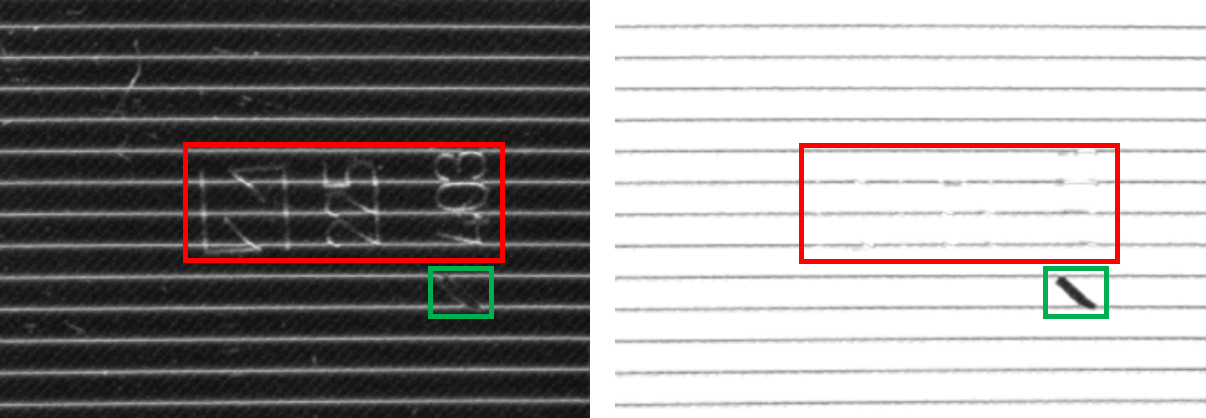
\includegraphics[width=\textwidth]{03_sichtpruefungDurchLichtstreuung/einsatzVonMehrerenStreifenmustern/figures/minAndMaxLink}
	\caption[Verknüpfte Bilder über Minimierung und Maximierung]{Verknüpfte Bilder, um Defekte von \textit{Fall 1} (rot umrahmt) und Defekte von \textit{Fall 2} (grün umrahmt) isoliert voneinander zu betrachten. Links über Minimierung und rechts über Maximierung verknüpft. Die verknüpften Quellbilder sind in Abbildung \ref{img:imageToLink} einzusehen.}
	\label{img:minAndMaxLink}
\end{figure}

\noindent
In den Bildern aus Abbildung \ref{img:minAndMaxLink} sind noch horizontale Streifen zu erkennen.
Diese sind keine Defekte, sondern entstehen aus Überlappungen der Streifenmuster in den Kamerabildern.
Auf diese \glqq Fehler\grqq ~und Möglichkeiten zur Beseitigung dieser wird im nächsten Abschnitt \ref{sec:optimierungen} ~eingegangen.

\p
Als Nächstes sollen beide Fälle in einem Gesamtbild kenntlich gemacht werden.
Hierfür macht man sich die Gemeinsamkeiten von \textit{Fall 1} und \textit{Fall 2} zunutze.
Man kann feststellen, dass die Helligkeit der Defekte in beiden Kamerabildern trotz Veränderung der Muster ungefähr gleich bleibt.
Verknüpft man die beiden Bilder durch die punktweise betragsmäßige Differenz, werden Defekte aus den beiden Fällen dunkel.
Die restliche, normal-spiegelnde Oberfläche wird hell, da jeder sonstige Bildpunkt in einem Muster dunkel und im anderen Muster hell erscheinen sollte, also eine hohe Differenz ergibt.
Die Ausnahme bilden dabei auch hier die Überlappungen der Streifen (siehe Abbildung \ref{img:diffImage}).

\begin{figure}[H]
	\centering
	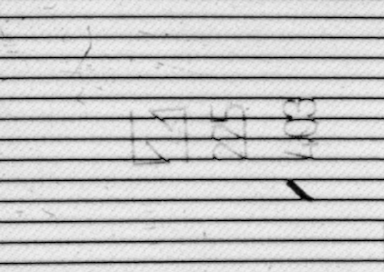
\includegraphics[width=0.5\textwidth]{03_sichtpruefungDurchLichtstreuung/einsatzVonMehrerenStreifenmustern/figures/diffImage}
	\caption[Verknüpfte Bilder über Differenz]{Über betragsmäßige Differenz verknüpfte Bilder.}
	\label{img:diffImage}
\end{figure}
}

%Optimierungen
{
	\FloatBarrier
    \section{Optimierungen}
    \label{sec:optimierungen}
    Nach dem Verknüpfen der Bilder verbleiben neben den Defekten noch schmale horizontale Streifen (vgl. Abbildung \ref{img:minAndMaxLink} und \ref{img:diffImage}).
Diese entstehen, wenn in den Kamerabildern von den um $\pi$ phasenverschobenen Streifenmustern Überlappungen der Streifen vorkommen.
Das kann durch eine Reihe von Ungenauigkeiten im gesamten Prozess passieren.
Zum besseren Verständnis muss auf die Differenzen zwischen dem aufgenommenen Kamerabild und der erzeugten Muster auf dem Bildschirm eingegangen werden.

% Unterschiede zwischen Kameraufnahme und Monitorbild
{
	\FloatBarrier
    \subsection{Unterschiede zwischen Kameraufnahme und Monitorbild}
    \label{sub:unterschiedeKameraUndMonitor}
    Das Kameraobjektiv hat bestimmte Einstellungsmöglichkeiten, darunter die Blende und der Fokus.
Aufgrund der festen Brennweite des verwendeten Objektivs wird der Einfluss der Brennweite nicht genauer betrachtet.
Die entscheidenden Einstellungen für diesen Prozess sind also der Fokus und die Blende.
Über die Fokussteuerung kann eine einzelne Tiefenebene im Bild scharf gestellt werden.
Da das Prüfobjekt und das Streifenmuster in unterschiedlichen Tiefenebenen liegen, führt das bereits dazu, dass im Kamerabild nicht beides gleichzeitig fokussiert werden kann.
Der Fokus liegt zur Prüfung auf der Oberfläche des Objekts.
Dadurch wird das Streifenmuster unscharf, wodurch die Breiten der hellen und dunklen Streifen verändert werden.
Die zweite Einstellungsmöglichkeit ist die Blende.
Öffnet man diese weiter, lässt man mehr Licht in den Kamerasensor.
Durch mehr einfallendes Licht vergrößern sich die Breiten der hellen Streifen im Bild.
Oberflächendefekte des Prüfobjekts werden gleichzeitig besser sichtbar.
Zur Kompensation der unterschiedlichen Streifenbreiten im Kamerabild müssen die Breiten der hellen und dunklen Streifen im erzeugten Muster unterschiedlich gewählt werden (siehe Abbildung \ref{img:differenceCamPat}).

\begin{figure}[H]
	\centering
	
\includegraphics[width=\textwidth]{03_sichtpruefungDurchLichtstreuung/optimierungen/unterschiedeKameraUndMonitor/figures/differenceCameraPattern}
	\caption[Unterschied zwischen Muster und Kameraaufnahme]{Unterschied zwischen Muster und Kameraaufnahme. Links erzeugtes Muster mit fünf Pixel Breite der hellen und neun Pixel Breite der dunklen Streifen, Rechts Kameraaufnahme}
	\label{img:differenceCamPat}
\end{figure}

\noindent
Man muss also mit Streifenmustern arbeiten, die von der Gleichung \ref{eq:rstreifenmuster} abweichen und unterschiedliche Breiten für die hellen und dunklen Streifen haben.
Es kommt dazu, dass die hellen und dunklen Streifen im Kamerabild unter Umständen nicht exakt gleich breit sein können, da die Anpassung der Streifenbreiten lediglich auf pixelgenauer Ebene durchgeführt werden kann.
Außerdem gibt es auch bei der Phase der Streifenmuster die Beschränkung, dass die maximale Genauigkeit der Verschiebung auch ein Pixel beträgt.
Das bedeutet, dass die Streifen selbst bei exakt gleicher Breite unter dem Kamerabild nicht genau versetzt voneinander liegen.
Es kommt hinzu, dass diese Genauigkeit sich auf den projizierenden Bildschirm bezieht.
Durch das Brillenglas zwischen der Kamera und dem Bildschirm kann die Phasenverschiebung im Kamerabild also mit zusätzlichen Fehlern behaftet sein.
Außerdem ist zu beachten, dass in der Kameraaufnahme stets ein Rauschen die Szene überlagert.
}

% Muster mit unterschiedlichen Breiten Streifenbreiten
{
	\FloatBarrier
    \subsection{Muster mit unterschiedlichen Streifenbreiten}
    \label{sub:musterUnterschiedlichenStreifenbreiten}
    Das erzeugte Streifenmuster in Abbildung \ref{img:differenceCamPat} hat nicht mehr den Grauwertverlauf einer Rechteckschwingung (vgl. Abbildung \ref{tikz:abbRechteckschwingung}) entlang der Ausbreitungsrichtung.
Dadurch lässt sich das Streifenmuster nicht mehr in der Form aus Gleichung \ref{eq:rstreifenmuster} darstellen.
Der Grauwertverlauf in einer Zeile bzw. Spalte eines solchen Streifenmusters entspricht einer Impulsschwingung (siehe Abbildung \ref{tikz:abbPulsewave}).
%
% Abbildung: Pulswave
{
	\begin{figure}[H]
		\centering
		\input{03_sichtpruefungDurchLichtstreuung/optimierungen/musterMitUnterschiedlichenStreifenbreiten/figures/abbPulsewave}
		\label{tikz:abbPulsewave}
	\end{figure}
}
%
\noindent
Um eine Gleichung für eine solche Impulsschwingung (siehe Abbildung \ref{tikz:abbPulsewave}) herzuleiten, kann man die periodische Sägezahnschwingung verwenden \cite{waveGeneration}.
Eine Sägezahnschwingung lässt sich darstellen durch (vgl. \cite{sawtoothWave}):
%
\begin{equation} \label{eq:saegezahnschwingung}
	w_f(t) = 2 \left( ft - \left\lfloor ft \right\rfloor \right) - 1
\end{equation}
%
\noindent
$f$ bezeichnet die Frequenz der Sägezahnschwingung und steht analog zu Gleichung \ref{eq:einheitsrechteckschwingung} über den Kehrwert im Zusammenhang mit der Periodenlänge der Sägezahnschwingung $w_f(t)$:
%
\begin{equation*}
	f = \dfrac{1}{T}
\end{equation*}
%
Mit $T = 3$ erhält man folgendes Schaubild (siehe Abbildung \ref{tikz:abbsaegezahnSchwingung}).
%
% Abbildung: Sägezahnschwingung
{
	\begin{figure}[H]
		\centering
		\input{03_sichtpruefungDurchLichtstreuung/optimierungen/musterMitUnterschiedlichenStreifenbreiten/figures/abbSaegezahnSchwingung}
		\label{tikz:abbsaegezahnSchwingung}
	\end{figure}
}
%
\noindent
Bildet man die Differenz von zwei zueinander um $\tfrac{D}{f}$  in $t$-Richtung versetzten Sä\-ge\-zahn\-funk\-ti\-onen, erhält man die Impulsschwingung $p_{f,D}(t)$:
%
\begin{equation} \label{eq:pulsewave}
	p_{f,D}(t) = w_f(t - \dfrac{D}{f}) - w_f(t) - w_f(- \dfrac{D}{f}),
	\quad
	D \in \left(0,1\right] \subset \acrshortmath{real}
\end{equation}
%
\noindent
$D$ wird Tastgrad (\textit{engl: duty cycle}) genannt und bezeichnet die Impulsdauer der Impulsschwingung im Verhältnis zur Periodenlänge $T$.
Auch für die Impulsschwingung gilt der Zusammenhang zwischen der Frequenz $f$ und der Periodendauer $T$ wie für die Sä\-ge\-zahn\-schwin\-gung:
%
\begin{equation*}
	f = \dfrac{1}{T}
\end{equation*}
%
Somit erhält man mit $D = \tfrac{1}{2}$ eine Rechteckschwingung wie auch in Abbildung \ref{tikz:abbRechteckschwingung}.
Ein Schaubild der Gleichung \ref{eq:pulsewave} wird in Abbildung \ref{tikz:abbNormalPulsewave} dargestellt.
%
% Abbildung: Normale Impulsschwingung
{
	\begin{figure}[H]
		\centering
		\input{03_sichtpruefungDurchLichtstreuung/optimierungen/musterMitUnterschiedlichenStreifenbreiten/figures/abbNormalPulsewave}
		\label{tikz:abbNormalPulsewave}
	\end{figure}
}
%
\noindent
Aus Gleichung \ref{eq:pulsewave} lässt sich somit eine mathematische Darstellung für Streifenmuster mit unterschiedlichen Streifenbreiten aufschreiben:
%
\begin{equation} \label{eq:impulsStreifenmuster}
	\begin{gathered}
		m_k(x,y) = A_m \left( 1 + p_{f,D}\left( x - \dfrac{1}{2 \pi f} \psi_k \right) \right),
		\\
		f = \dfrac{N_p}{\acrshortmath{lwidth}},
		\quad
		D \in \left(0,1\right] \subset \acrshortmath{real},
		\quad
		\psi_k = (k - 1)\dfrac{2\pi}{N_{shift}},
		\quad
		k \in \lbrace 1,\ldots,N_{shift}\rbrace
	\end{gathered}
\end{equation}
%
Wie auch in Gleichung \ref{eq:rstreifenmuster} gilt für dieses Muster die Periodizität in der Ausbreitungsrichtung.
Auch hier bezeichnet $A_m$ die Amplitude, $N_p$ die Anzahl der Perioden über die Monitorbreite \acrshort{lwidth}, $N_{shift}$ die Anzahl der Phasenverschiebungen und $\psi_k$ die Phasenverschiebung des $k$-ten Musters.
Zusätzlich zu diesen Parametern hat man den Tastgrad $D$, der in diesem Fall die Breite der hellen Streifen im Verhältnis zu der Periodenlänge $T$ angibt.
Die Periodenlänge $T$ ist im Streifenmuster die Summe der Breite eines einzelnen dunklen und eines einzelnen hellen Streifens.
Analog zu Gleichung \ref{eq:impulsStreifenmuster} lässt sich auch ein horizontales Streifenmuster mit Ausbreitungsrichtung in $y$ über die Monitorhöhe \acrshort{lheight} beschreiben.
Das Bild eines horizontalen Streifenmusters analog zu Gleichung \ref{eq:impulsStreifenmuster}, d. h. mit Ausbreitungsrichtung in $y$, wird in Abbildung \ref{tikz:abbImpulsStreifenmuster} dargestellt.
%
% Abbildung: Impuls-Streifenmuster
{
	\begin{figure}[H]
		\centering
		\input{03_sichtpruefungDurchLichtstreuung/optimierungen/musterMitUnterschiedlichenStreifenbreiten/figures/abbImpulsStreifenmuster}
		\label{tikz:abbImpulsStreifenmuster}
	\end{figure}
}
}

% Verknüpfung mehrerer Kameraaufnahmen
{
	\FloatBarrier
    \subsection{Verknüpfung mehrerer Kameraaufnahmen}
    \label{sub:verknuepfungMehrererKameraaufnahmen}
    Da die Kameraeinstellungen auf die Prüfstation und Prüfbedingungen angepasst werden müssen, sind die Möglichkeiten zur Eliminierung der Streifen im Vorhinein begrenzt.
Die Nachbearbeitung kann über verschiedene Ansätze erfolgen.
Aufgrund der Periodizität und der festen Ausbreitungsrichtung der Streifen bietet es sich an, die Fourier-Analyse anzuwenden.
Man untersucht die Frequenzkomponenten der Streifen und filtert speziell diese aus dem Bild heraus, um sie zu entfernen.
Diese Methode kann allerdings nicht die fehlende Information an den dunklen Streifen wiederherstellen, sondern lediglich eine Bildverbesserung durchführen.
Eine andere Möglichkeit ist das Hinzuziehen von weiteren Bildern.
Da an den Stellen der horizontalen Streifen die Information fehlt, kann man zusätzliche Muster zur Hand nehmen, um die Informationen zu ergänzen.
Man zieht weitere phasenverschobene Muster hinzu, sodass man eine gerade Anzahl an Phasenverschiebungen hat.
Daraus kann man die Informationen vereinen und eliminiert die Streifen, welche durch Überlappungen der versetzen Streifen in den Kamerabildern entstehen.
Im Folgenden werden als Beispiel die vier Kamerabilder der Streifenmustern $m_1 - m_4$ miteinander verknüpft, die mit $N_{shift} = 4$ gebildet wurden.
Aus den vier aufgenommenen Bildern verknüpft man je zwei Bilder mit der betragsmäßigen Differenz, in denen die Streifenmuster eine Phasenverschiebung von $\pi$ zueinander haben.
Die zwei resultierenden Bilder haben zueinander versetzte Streifen, die aus den Überlappungen entstehen.
Zum Schluss kann man die beiden Bilder so verknüpfen, dass man stets den Bildpunkt mit dem höheren Helligkeitswert nimmt.
Das entspricht der Maximierung.
Analog kann man auch die horizontalen Streifen aus Abbildung \ref{img:minAndMaxLink} eliminieren, in welcher die Typen von Fehlstellen isoliert voneinander betrachtet wurden.
In Abbildung \ref{img:imageTree} werden die einzelnen Schritte dieses Verfahrens veranschaulicht.
Analog lässt sich auch die Verknüpfung von mehr als vier phasenverschobenen Streifenmustern durchführen.

\begin{figure}[H]
	\centering
	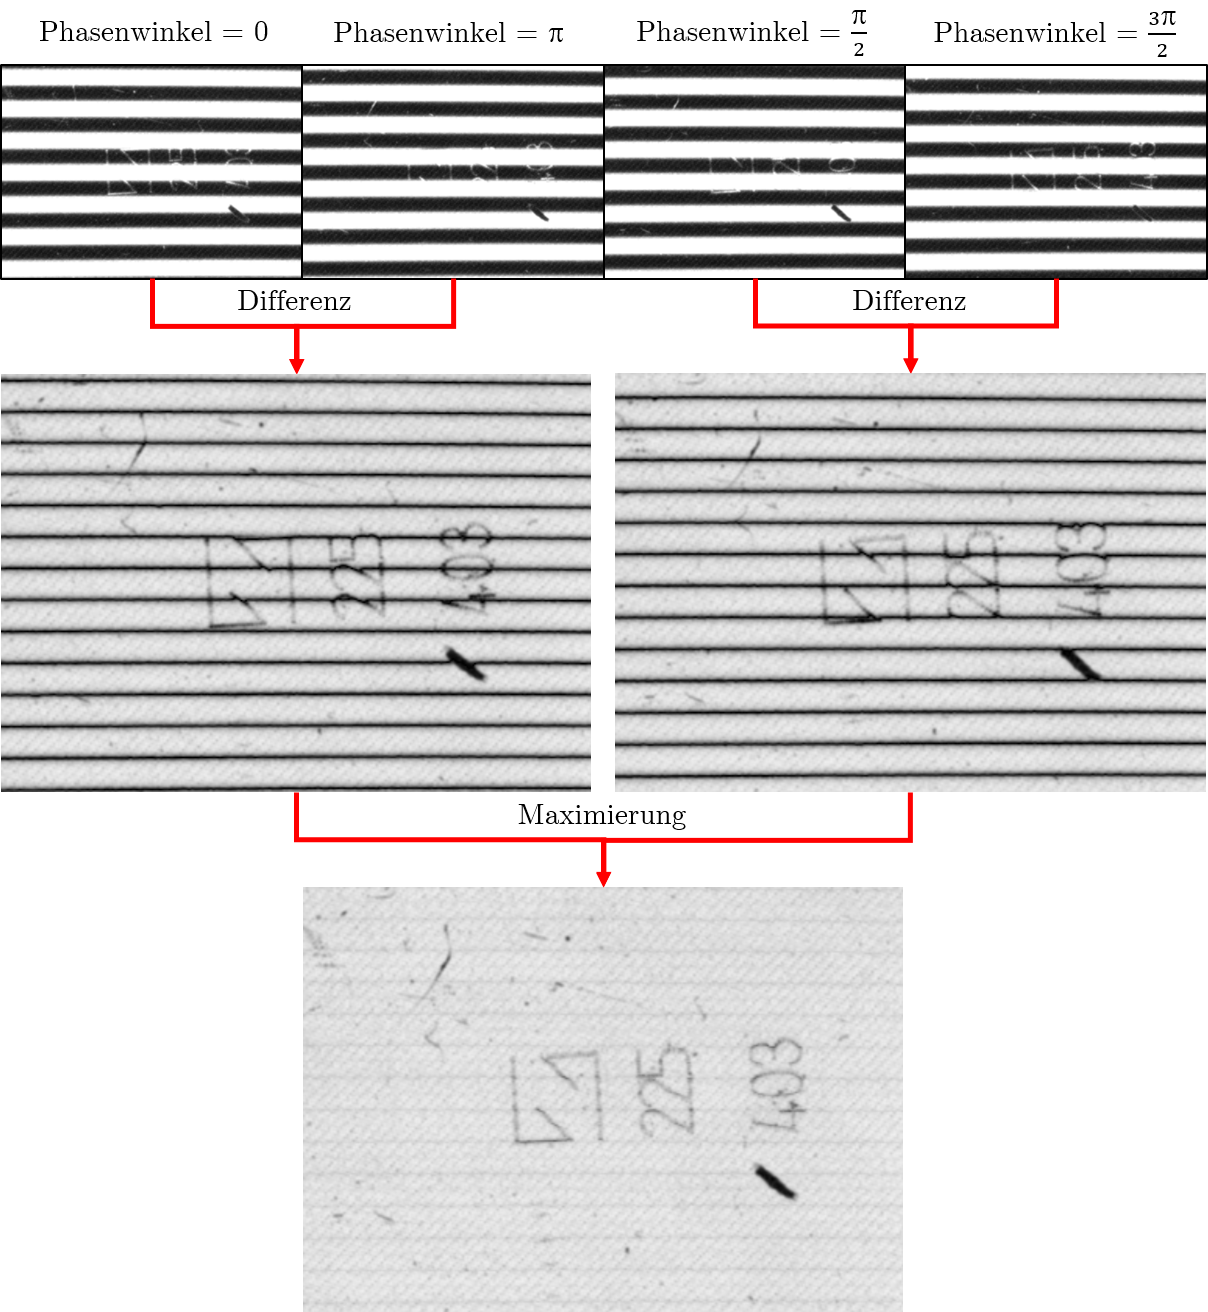
\includegraphics[width=\textwidth]{03_sichtpruefungDurchLichtstreuung/optimierungen/figures/imageTree}
	\caption[Prozess der Hervorhebung von Oberflächendefekten]{Prozess zur Hervorhebung von Oberflächendefekten mit $N_{shift} = 4$.}
	\label{img:imageTree}
\end{figure}
}

% Nachbearbeitung mit der Fourier-Analyse
{
	\FloatBarrier
    \subsection{Nachbearbeitung mit der Fourier-Analyse}
    \label{sub:nachbearbeitungFourierAnalyse}
    \noindent
Im praktischen Durchlauf verbleiben auch im letzten Bild noch sehr schwache horizontale Streifen.
Das liegt an den oben genannten Ungenauigkeiten im Prüfprozess und der Mustererzeugung.
Da das Ergebnis mit weiteren phasenverschobenen Streifenmustern stetig besser wird, könnte man diese durch eine höhere Anzahl von Streifenmustern $N_{shift}$ eliminieren.
Dabei gilt zu beachten, dass man im Diskreten arbeitet und bei einer sehr hohen Anzahl von Phasenverschiebungen Messfehler und Gleitpunktfehler zum Tragen kommen.
Das bedeutet, man muss eine zum Prüfaufbau passende Anzahl an Mustern verwenden, um bessere Ergebnisse dokumentieren zu können.
Zur Bildverbesserung hat man aber auch die Möglichkeit, die zuvor erwähnte Fourier-Analyse anzuwenden.
Die noch verbliebenen Strukturen lassen sich im Amplitudenspektrum des Bildes durch die Ausbreitungsrichtung finden.
Da diese Strukturen nur noch sehr schwach im Bild vorhanden ist, sind die jeweiligen Frequenzkomponenten auch dementsprechend gering gewichtet (siehe Abbildung \ref{img:amplitudeSpectrum}).

\begin{figure}[H]
	\centering
	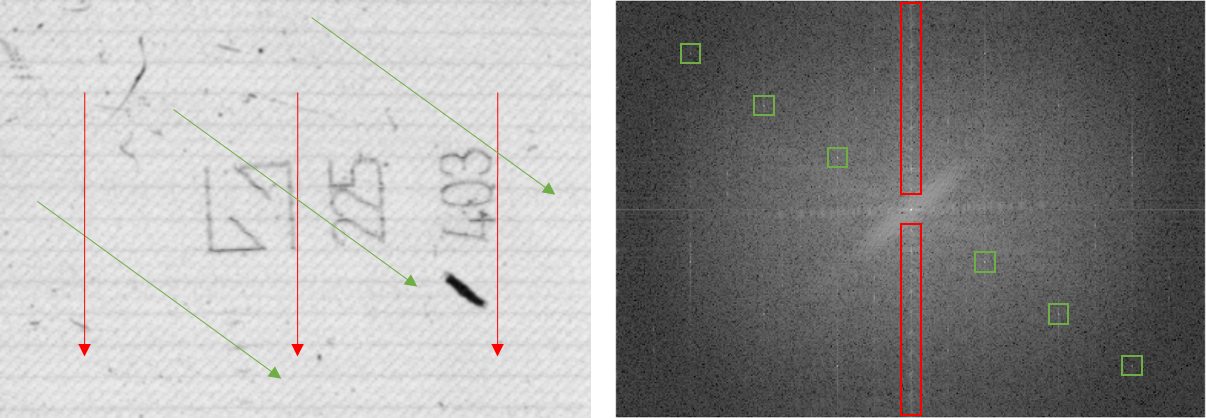
\includegraphics[width=\textwidth]{03_sichtpruefungDurchLichtstreuung/optimierungen/figures/amplitudeSpectrum}
	\caption[Amplitudenspektrum des Gesamtbildes]{Amplitudenspektrum des Gesamtbildes. (mit Markierungen)}
	\label{img:amplitudeSpectrum}
\end{figure}

\noindent
In Rot ist im Bild die Ausbreitungsrichtung der ersten Struktur markiert, die entsprechenden Gewichte der Frequenzkomponenten sind in derselben Farbe im Amplitudenspektrum gezeichnet.
Analog sind in Grün die für die zweite Struktur relevante Ausbreitungsrichtung und Gewichte der Frequenzkomponenten markiert.
Filtert man im Amplitudenspektrum die markierten Bereiche heraus und wendet die inverse Fourier-Transformation an, erhält man ein Bild, indem die beiden störenden Strukturen nicht mehr vorhanden sind.
Das Ergebnisbild wird durch ein geeignetes Online-Werkzeug \cite{fourierTool} berechnet und in Abbildung \ref{img:frequencyFiltered} dargestellt.

\begin{figure}[H]
	\centering
	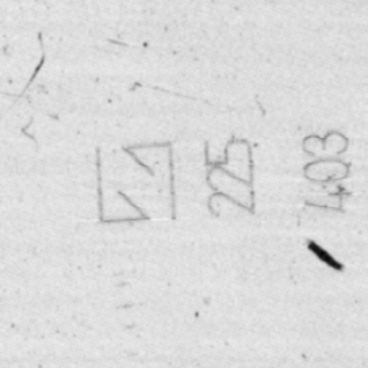
\includegraphics[width=0.4\textwidth]{03_sichtpruefungDurchLichtstreuung/optimierungen/figures/frequencyFiltered}
	\caption[Bild mit angewandtem frequenzselektives Filter]{Angewandtes frequenzselektives Filter nach Abbildung \ref{img:amplitudeSpectrum}. Erstellt mit dem Online-Werkzeug \glqq Fourifier\grqq ~von © 2020 Ejectamenta.\cite{fourierTool}\footnotemark}
	\label{img:frequencyFiltered}
\end{figure}
\footnotetext{Anmerkungen: Das Bild musste aufgrund der Anforderungen des verwendeten Online-Werkzeugs zugeschnitten werden. Außerdem wurden die Frequenzkomponenten \glqq händisch\grqq ~entfernt, weshalb das Bild fehlerbehaftet ist. Das Bild konnte auch nicht auf Korrektheit geprüft werden und dient nur der Veranschaulichung. Die Nutzungsrechte unterliegen der Lizenz von © 2020 Ejectamenta. Für weitere Informationen zu Geschäfts- und Nutzungsbedingungen siehe: \url{https://ejectamenta.com/about/terms-of-service/}}
}

\noindent
Mit dem vorgestellten deflektometrischen Verfahren wurden Oberflächendefekte wie z. B. Kratzer, Eingravierungen oder Partikel auf transparenten und spiegelnden Prüfobjekten sichtbar gemacht.
Das erzeugte Gesamtbild dieses Verfahrens kann nun durch anschließende Bildverarbeitung analysiert und geprüft werden.
In diesem konkreten Fall würden sich z. B. Kratzer detektieren oder die eingravierten Zeichen auslesen lassen.

\p
Dieses Verfahren kann je nach Parametrisierung mit unterschiedlicher Empfindlichkeit Abweichungen, die die Lichtreflexionen beeinflussen, in der Oberfläche sichtbar machen.
Dadurch eignet es sich besonders für Brillengläser und transparente Objekte.
Für spiegelnde Objekte mit einem angepasstem Aufbau konnten ähnliche Ergebnisse erzielt werden, allerdings treten nochmal größere Schwankungen in den Streifenbreiten auf.
Diese müssen durch eine größere Anzahl an Bildaufnahmen kompensiert werden.
Das Verfahren ist außerdem auf Kratzer und Eingravierungen optimiert.
Für spiegelnde Objekte empfiehlt sich aus dem Grund ein anderes Verfahren, das im Kapitel \ref{chp:deflektometrischeRegistrierung} beschrieben wird.
}
	}
	
	%Deflektometrische Registrierung
	{
		\FloatBarrier %Verhindert Fehlpositionierung von Abbildungen aus vorherigen Abschnitten
		\chapter{Deflektometrische Registrierung}
		\label{chp:deflektometrischeRegistrierung}
		\begin{Definition}{Deflektometrische Registrierung}{def:deflektometrischeRegistrierung}
	Die \textit{deflektometrische Registrierung} \acrshort{lr} beschreibt die Abbildung von Bildpunkten zu Schirmpunkten. \cite{kit_werling}
	%
	\begin{equation*}
		\acrshortmath{lr} : A_{Cam} \rightarrow L \cup \varnothing ,\quad P_{B} \rightarrow P_{L}
	\end{equation*}
	%
	$ A_{Cam} \subset \mathbb{R}^{2} $ bezeichnet die Menge der Bildpunkte bzw. der Kamerapixel.
	$ L \subset \mathbb{R}^{2} $ bezeichnet die Menge der Schirmpunkte bzw. der Monitorpixel.
	In Koordinatenschreibweise lässt sich die Abbildung somit darstellen als:
	%
	\begin{equation*}\label{eq:deflektometrischeRegistrierungAbbildung}
		\acrshortmath{lr} : \mathbb{R}^{2} \supset A_{Cam} \rightarrow \mathbb{R}^2 ,\quad (x_{B}, y_{B}) \mapsto (x_{L}, y_{L})
	\end{equation*}
\end{Definition}

\begin{Satz}{Separierbarkeit der deflektometrischen Registrierung}{theo:separierbarkeitDeflektometrischeRegistrierung}
Ferner kann die \textit{deflektometrische Registrierung} \acrshort{lr} in zwei Abbildungen von Bildpunkten zu den Spalten- und Zeilenpositionen der Schirmpunkte separiert werden:
	%
	\begin{equation*}
		\acrshortmath{lrx} : \mathbb{R}^{2} \supset A_{Cam} \rightarrow \mathbb{R} ,\quad (x_{B}, y_{B}) \mapsto x_{L}
	\end{equation*}
	%
	\begin{equation*}
		\acrshortmath{lry} : \mathbb{R}^{2} \supset A_{Cam} \rightarrow \mathbb{R} ,\quad (x_{B}, y_{B}) \mapsto y_{L}
	\end{equation*}
	%
\end{Satz}

\noindent
Die deflektometrische Registrierung kann aus der Beobachtung des Monitors mithilfe der Kamera aufgestellt werden.
Wird der Monitor indirekt über eine spiegelnde Oberfläche beobachtet, können aus der deflektometrischen Registrierung Krümmungsmerkmale über die spiegelnde Oberfläche bestimmt werden.
Durch die Berücksichtigung der Positionen der Systemkomponenten können mittels der deflektometrischen Registrierung Höheninformationen über die Oberfläche gewonnen werden.
Dieses Verfahren wurde im Abschnitt \ref{sub:rekonstruktion} bereits beschrieben.

%Bestimmung der deflektometrischen Registrierung
{
	\FloatBarrier
    \section{Bestimmung der deflektometrischen Registrierung}
    \label{sec:bestimmungDeflektometrischeRegistrierung}
    Die Bestimmung der deflektometrischen Registrierung nach Definition \ref{def:deflektometrischeRegistrierung} bedeutet eine Zuordnung von Kamerapixeln zu Monitorpixeln.
Grundsätzlich soll jeder Lichtstrahl, der über das Prüfobjekt in die Kamera reflektiert wird im Kamerabild identifizierbar sein.
Eine einfache Möglichkeit eine solche Zuordnung zu erreichen bekommt man, indem man die Pixel des Monitors einzeln einschaltet und dabei die Veränderung im Kamerabild betrachtet.
Bei kleinen Bildern ist dies noch umsetzbar, allerdings wird die Anzahl von Pixeln mit zunehmender Auflösung schnell sehr groß und unübersichtlich, sodass dieser Ansatz nicht praktikabel ist.
Aus dem Grund ist es effektiver Bilder auf dem Monitor anzuzeigen, die Positionen visuell codieren können.
Durch die visuelle Erfassung des Spiegelbilds können somit die zugehörigen Positionen auf dem Monitor berechnet werden.

\p
Ein herkömmliches Kodierverfahren für solche Prozesse ist das Phasenschiebeverfahren.
Der Ansatz bei dem Verfahren ist es die Zeilen- und Spaltenpositionen des Monitors durch periodische Muster zu kodieren.
Die Grauwerte von periodischen Mustern nehmen dabei Werte an, die über die periodische Funktion bestimmt wurden.
Die hier verwendeten Funktionen sind Kosinusfunktionen.
Damit können die Pixel des Musters Phaseninformationen eines lokalen Orts übertragen.
Durch die Periodizität der Funktionen kann aus der reinen Phaseninformation noch nicht die genaue Monitorposition bestimmt werden.
Die Lösung dieses Problems wird als Phasenentfaltung bezeichnet (siehe auch Definition \ref{def:phasenentfaltung}).
Hierzu stellt Werling in seiner Arbeit \cite{kit_sbw} ein mehrstufiges Phasenschiebeverfahren vor, das Muster mit unterschiedlichen Perioden verwendet.

\begin{Definition}{Phasenentfaltung}{def:phasenentfaltung}
	Die \textit{Phasenentfaltung} bezeichnet den Vorgang zur Auflösung der mehrdeutigen Zuordnung der Phaseninformation.
\end{Definition}

%Deflektometrische Registrierung ohne Phasenentfaltung
{
	\FloatBarrier
    \subsection{Deflektometrische Registrierung ohne Phasenentfaltung}
    \label{sub:registrierungOhnePhasenentfaltung}
    Ohne eine Phasenentfaltung bekommt man eventuell eine mehrdeutige Zuordnung aufgrund der Periodizität der Kosinusfunktion.
Soll eine eindeutige Zuordnung über das Phasenschiebeverfahren ohne Phasenentfaltung erfolgen, darf es also nur eine einzige Musterperiode auf der Monitorbreite bzw. Monitorhöhe geben.
Damit lässt sich die Kodierung der Monitorkoordinaten $(x_{L}, y_{L})$ durch die Phasen $(\phi_{x}, \phi_{y})$ folgendermaßen aufstellen:
%
\begin{equation}\label{eq:phasenkodierung}
	x_{L} = \dfrac{\text{\acrshort{lwidth}}}{2\pi}\phi_{x},
	\qquad
	y_{L} = \dfrac{\text{\acrshort{lheight}}}{2\pi}\phi_{y}
\end{equation}
%
\noindent
Die Monitorbreite wird dabei mit \acrshort{lwidth} und die Monitorhöhe mit \acrshort{lheight} angegeben.

\p
O.B.d.A. wird nachfolgend nur die deflektometrische Registrierung der Spaltenpositionen \acrshort{lrx} ($x$-Richtung) betrachtet.
Die deflektometrische Registrierung der Zeilenpositionen \acrshort{lry} ($y$-Richtung) kann analog bestimmt werden.
Das $k$-te Muster $m_k$ zur Kodierung der Monitorpunkte wird durch eine Kosinusfunktion aufgebaut und hat die Form:
%
\begin{equation}\label{eq:monitormuster}
	\begin{split}	
		m_k(x_L,y_L) = A_m \left(1 + C_m \cos \left(\dfrac{2\pi}{\text{\acrshort{lwidth}}} x_L + \psi_k\right)\right),
		\qquad
		k \in \lbrace 1,\ldots,N_{shift}\rbrace, \\
		\psi_k = (k - 1)\dfrac{2\pi}{N_{shift}}
	\end{split}
\end{equation}
%
$A_m$ bezeichnet die Amplitude, $C_m$ den Kontrast, $\psi_k$ die Phasenverschiebung des $k$-ten Musters und $N_{shift}$ die Anzahl an Mustern für das Phasenschiebeverfahren.
Das Muster wird auf dem Monitor angezeigt und über eine spiegelnde Oberfläche durch die Kamera beobachtet.
Über die Reflexion an der Oberfläche trifft der Sichtstrahl ausgehend vom Bildpunkt $(x_B, y_B)^\top \in A_{Cam}$ den Monitor im Punkt $(x_L, y_L)^\top \in L \cup \varnothing$ bestimmt durch die Abbildung aus der Gleichung \ref{eq:deflektometrischeRegistrierungAbbildung}:
%
\begin{equation}
	\begin{pmatrix}
		x_L \\ 
		y_L
	\end{pmatrix}
	= \text{\acrshort{lr}}(x_B, y_B) = 
	\begin{pmatrix}
		\text{\acrshort{lrx}}(x_B, y_B) \\ 
		\text{\acrshort{lry}}(x_B, y_B)
	\end{pmatrix} 
\end{equation}
%
Dementsprechend lässt sich das $k$-te Kamerabild $g$ am Bildpunkt $(x_B, y_B)^\top$ beschreiben durch das $k$-te Muster am Punkt $\text{\acrshort{lrx}}(x_B, y_B), \text{\acrshort{lry}}(x_B, y_B))^\top$:
%
\begin{equation}
	g_k(x_B, y_B) = m_k(\text{\acrshort{lrx}}(x_B, y_B), \text{\acrshort{lry}}(x_B, y_B))
\end{equation}
%
Setzt man für $m_k$ die Gleichung \ref{eq:monitormuster} unter Berücksichtigung der Veränderung durch die Oberfläche erhält man:
%
\begin{equation}\label{eq:kamerabild}
	g_k(x_B, y_B) = A_g(x_B, y_B) \left(1 + C_g(x_B, y_B) \cos \left(\dfrac{2\pi}{\text{\acrshort{lwidth}}}\text{\acrshort{lrx}}(x_B, y_B) + \psi_k\right)\right)
\end{equation}
%
Dabei sind die Amplitude $A_g$ und der Kontrast $C_g$ des Musters im Kamerabild unter Umständen unterschiedlich zu dem angezeigten Muster im Monitorbild.
Der Unterschied ist abhängig von dem Oberflächenpunkt an dem der Sichtstrahl reflektiert wird.
Aus dem Grund werden $A_g$ und $C_g$ in Abhängigkeit vom Kamerabildpunkt $(x_B, y_B)^\top$ angegeben.

\p
Durch Umstellung der Gleichung \ref{eq:phasenkodierung} nach der Phase und Einsetzen der deflektometrischen Registrierung \acrshort{lr}, erhält man die Phase $\phi_x$ des $k$-ten Musters in Abhängigkeit von den Kamerabildpunkten:
%
\begin{equation}\label{eq:phaseBildkoordinaten}
	\phi_x = \dfrac{2\pi}{\text{\acrshort{lwidth}}}\text{\acrshort{lrx}}(x_B, y_B)
\end{equation}
%
Durch Einsetzen der Phase aus Gleichung \ref{eq:phaseBildkoordinaten} in die Gleichung \ref{eq:kamerabild} des Kamerabilds erhält man den Zusammenhang zwischen der Phase $\phi_x$ des $k$-ten Musters und dem Kamerabild   $g_k$:
%
\begin{equation}\label{eq:kamerabildMitPhase}
	g_k(x_B, y_B) = A_g(x_B, y_B) \left(1 + C_g(x_B, y_B) \cos \left(\phi_x(x_B, y_B) + \psi_k\right)\right)
\end{equation}
%
Unter Einbeziehung der $N_{shift}$-vielen phasenverschobenen Streifenmuster kann man die Phase $\phi_x$ berechnen:
%
\begin{equation}\label{eq:tanPhase}
	\tan (\phi_x) = -\dfrac{\sum\limits_{k=1}^{N_{shift}} g_k(x_B, y_B) sin(\psi_k)}{\sum\limits_{k=1}^{N_{shift}} g_k(x_B, y_B) cos(\psi_k)}
\end{equation}
%
Aus den Gleichungen \ref{eq:phasenkodierung} und \ref{eq:tanPhase} folgt schließlich:
%
\begin{equation}\label{eq:registrierungX}
	x_L = \text{\acrshort{lrx}}(x_B, y_B) = 
	\dfrac{\text{\acrshort{lwidth}}}{2\pi}
	\arctan 
	\left( 
		-\dfrac
		{\sum\limits_{k=1}^{N_{shift}} g_k(x_B, y_B) sin\left((k - 1)\dfrac{2\pi}{N_{shift}}\right)}
		{\sum\limits_{k=1}^{N_{shift}} g_k(x_B, y_B) cos\left((k - 1)\dfrac{2\pi}{N_{shift}}\right)}
	\right)
\end{equation}
%
Mittels der Gleichung \ref{eq:registrierungX} ist somit die deflektometrische Registrierung in $x$-Richtung angegeben und die Monitorpositionen eindeutig bestimmt.
Die deflektometrische Registrierung in $y$-Richtung lässt sich analog dazu bestimmen.
Die Anzahl an Mustern bzw. Phasenverschiebungen $N_{shift}$ ist noch als Parameter übrig geblieben.
Um eine eindeutige Zuordnung zu erhalten, benötigt man aufgrund der drei unbekannten Größen Amplitude $A_g$, Kontrast $C_g$ und Phase $\phi_x$ in Gleichung \ref{eq:kamerabildMitPhase} eine Mindestanzahl von drei Phasenverschiebungen.

\p
Durch die Eindeutigkeit der Phase in dem verwendeten Muster spart man sich die Phasenentfaltung.
Dennoch ist das Phasenschiebeverfahren nach diesem Ansatz nicht sehr präzise und daher eher ungeeignet für Praxisanwendungen.
Der Grund liegt darin, dass Monitore lediglich eine vergleichsweise kleine Anzahl an Helligkeitsstufen darstellen können.
Die Anzahl an zu kodierenden Pixelpositionen sind in der Regel deutlich größer.
Eine ähnliche Beschränkung gibt es auch bei der Bildaufnahme, denn auch die Kamera nimmt eine Quantisierung vor und kann nicht sämtliche Helligkeitsstufen aufnehmen.
Zusammengenommen ist die Auflösung der Monitorpunkte damit stark begrenzt.
Eine höhere Ortsauflösung lässt sich erreichen indem man Muster mit mehreren Perioden über die Monitorbreite bzw. Monitorhöhe verwendet.
Damit wird schließlich eine Phasenentfaltung als zusätzliche Aufgabe erforderlich.
}
}

%Auswertung der deflektometrischen Registrierung
{
	\FloatBarrier
    \section{Auswertung der deflektometrischen Registrierung}
    \label{sec:auswertungDeflektometrischeRegistrierung}
    Die deflektometrische Registrierung \acrshort{lr} kann nicht ohne Weiteres direkt ausgewertet werden.
Deshalb wird im Folgenden die Weiterverarbeitung der deflektometrischen Registrierung beschrieben, sodass bekannte Methoden aus dem Gebiet der Bildverarbeitung angewendet werden können.

\p
Die graphische Darstellung der deflektometrischen Registrierung \acrshort{lr} stellt sich zunächst als schwierig heraus, da man mit einer Abbildung der Form $\acrshortmath{real}^2 \rightarrow \acrshortmath{real}^2$ arbeitet.
Aus dem Grund wird die Separierbarkeit der deflektometrischen Registrierung aus Satz \ref{theo:separierbarkeitDeflektometrischeRegistrierung} angewendet.
Daraus erhält man die beiden Abbildungen der Form $\acrshortmath{real}^2 \rightarrow \acrshortmath{real}$:
%
\begin{equation*}
	\acrshortmath{lrx} : \acrshortmath{real}^{2} \supset A_{Cam} \rightarrow \acrshortmath{real} ,\quad (x_{B}, y_{B}) \mapsto x_{L}
\end{equation*}
%
\begin{equation*}
	\acrshortmath{lry} : \acrshortmath{real}^{2} \supset A_{Cam} \rightarrow \acrshortmath{real} ,\quad (x_{B}, y_{B}) \mapsto y_{L}
\end{equation*}
%
In der Form lässt sich die Analogie zu der mathematischen Beschreibung eines Graubildes $f$ erkennen:
%
\begin{equation*}
	f : \acrshortmath{real}^{2} \supseteq [x_{min},x_{max}] \times [y_{min},y_{max}] \rightarrow [I_{min},I_{max}] \subseteq \acrshortmath{real} ,\quad (x,y) \mapsto f(x,y)
\end{equation*}
%
Für die Darstellung als Bilder sind somit lediglich geeignete Transformationen der Wertemengen der deflektometrischen Registrierungen \acrshort{lrx} und \acrshort{lry} nötig.
%
\begin{Definition}{Darstellung der Deflektometrischen Registrierung}{def:graphDeflektometrischeRegistrierung}
	Die deflektometrischen Registrierung \acrshort{lr} kann als zwei einzelne Graubilder \acrshort{frx} und \acrshort{fry} dargestellt werden.
	%	
	\begin{equation*}
		\acrshortmath{frx} : \acrshortmath{real}^2 \supset \acrshortmath{d}(\acrshortmath{lrx}) \rightarrow [I_{min},I_{max}] \subseteq \acrshortmath{real}
	\end{equation*}
	%
	\begin{equation*}
		\acrshortmath{fry} : \acrshortmath{real}^2 \supset \acrshortmath{d}(\acrshortmath{lry}) \rightarrow [I_{min},I_{max}] \subseteq \acrshortmath{real}
	\end{equation*}
	%
	Die Bilder \acrshort{frx} und \acrshort{fry} sind definiert durch:
	%	
	\begin{equation*}
		\acrshortmath{frx}(x,y) := t_x(\acrshortmath{lrx}(x,y))
	\end{equation*}
	%	
	\begin{equation*}
		\acrshortmath{fry}(x,y) := t_y(\acrshortmath{lry}(x,y))
	\end{equation*}
	%
	Mit $\acrshortmath{d}(\acrshortmath{frx}) = \acrshortmath{d}(\acrshortmath{lrx})$ und $\acrshortmath{d}(\acrshortmath{fry}) = \acrshortmath{d}(\acrshortmath{lry})$ und
	%
	\begin{equation*}
		t_x : \acrshortmath{real} \supset \acrshortmath{w}(\acrshortmath{lry}) \rightarrow [I_{min},I_{max}] \subseteq \acrshortmath{real}
	\end{equation*}
	%
	\begin{equation*}
		t_y : \acrshortmath{real} \supset \acrshortmath{w}(\acrshortmath{lry}) \rightarrow [I_{min},I_{max}] \subseteq \acrshortmath{real}
	\end{equation*}
	%
	Die Transformationen $t_x$ und $t_y$ sind definiert als:
	%	
	\begin{equation*}
		t_x(x) := \left(\dfrac{x}{\acrshortmath{lwidth}}(I_{max} - I_{min})\right) + I_{min}
	\end{equation*}
	%	
	\begin{equation*}
		t_y(y) := \left(\dfrac{y}{\acrshortmath{lheight}}(I_{max} - I_{min})\right) + I_{min}
	\end{equation*}
	%
\end{Definition}
%
Die Abbildungen $t_x$ und $t_y$ sind dabei lineare Transformationen der Wertemengen der deflektometrischen Abbildungen in Spalten und Zeilen zu den zulässigen Intensitäten für die Bilder \acrshort{frx} und \acrshort{fry}, angegeben durch das Intervall $[I_{min},I_{max}]$.

\p
Erstellt man aus der berechneten deflektometrischen Registrierung \acrshort{lr} einer ungekrümmten Fläche die zugehörigen Bilder \acrshort{frx} und \acrshort{fry} nach Definition \ref{def:graphDeflektometrischeRegistrierung}, erhält man Darstellungen wie in Abbildung \ref{tikz:abbOptimaleSpaltenZeilenReg}:

% Abbildung: Optimale Spalten- und Zeilenregistrierung
{
	\begin{figure}[H]
		\centering
		\begin{adjustbox}{width=\textwidth}
	\begin{tikzpicture}[every node/.style={inner sep=0,outer sep=0}]
	
		\node [anchor=north west] (imgSpalten) at (0,0) {
\includegraphics[width=.47\textwidth]{04_deflektometrischeRegistrierung/auswertungDeflektometrischeRegistrierung/figures/spaltenRegistrierung_optimal}};
		\node [below=0.2cm of imgSpalten] {Graubild der Spaltenzuordnung \acrshort{frx}$(x,y)$};
		\node [anchor=north west] (imgZeilen) at (0.53\textwidth,0) {
\includegraphics[width=.47\textwidth]{04_deflektometrischeRegistrierung/auswertungDeflektometrischeRegistrierung/figures/zeilenRegistrierung_optimal}};
		\node [below=0.2cm of imgZeilen] {Graubild der Zeilenzuordnung \acrshort{fry}$(x,y)$};
	
	\end{tikzpicture}
\end{adjustbox}
\caption[Darstellung Spalten- und Zeilenregistrierung]{Darstellung der Spalten- und Zeilenregistrierung als Bilder in Graustufen mit $I_{min} = 0$ und $I_{max} = 255$. Je dunkler ein Pixel ist, desto weiter links bzw. oben befindet sich die zugeordnete Spalten- bzw. Zeilenposition.}
		\label{tikz:abbOptimaleSpaltenZeilenReg}
	\end{figure}
}

\noindent
In Abbildung \ref{tikz:abbOptimaleSpaltenZeilenReg} wird direkt das Muster auf dem Monitor betrachtet.
Aus dem Grund lässt sich erkennen, dass die Zuordnung von Monitor- und Kamerapixeln in den Spalten und Zeilen linear verläuft.
Werden nun die Streifen durch besondere Oberflächeneigenschaften gekrümmt oder verzerrt, dann werden an diesen Stellen in den Bildern der deflektometrischen Registrierung Abweichungen vom linearen Grauwerteverlauf sichtbar.

% Abbildung: Brillenglas Registrierung
{
	\begin{figure}[H]
		\centering
		\begin{adjustbox}{width=\textwidth}
	\begin{tikzpicture}[every node/.style={inner sep=0,outer sep=0}]
	
		\node [anchor=north west] (imgSpalten) at (0,0) {\includegraphics[width=.47\textwidth]{04_deflektometrischeRegistrierung/auswertungDeflektometrischeRegistrierung/figures/streifenKrümmung_spalten}};
		\node [below=0.2cm of imgSpalten] {Graubild der Spaltenzuordnung \acrshort{frx}$(x,y)$};
		\node [anchor=north west] (imgZeilen) at (0.53\textwidth,0) {\includegraphics[width=.47\textwidth]{04_deflektometrischeRegistrierung/auswertungDeflektometrischeRegistrierung/figures/streifenKrümmung_zeilen}};
		\node [below=0.2cm of imgZeilen] {Graubild der Zeilenzuordnung \acrshort{fry}$(x,y)$};
	
	\end{tikzpicture}
\end{adjustbox}
\caption[Darstellung verzerrter Spalten- und Zeilenregistrierung]{Darstellung verzerrter Spalten- und Zeilenregistrierung als Bilder. Verzerrungen entstehen durch tiefe Eingravierungen im Glas.}
		\label{tikz:abbBrillenglasRegistrierung}
	\end{figure}
}

\noindent
Die deflektometrische Registrierung macht bestimmte Fehlstellen als Abweichung vom stetigen linearen Grauwertverlauf kenntlich (siehe Abbildung \ref{tikz:abbBrillenglasRegistrierung}).
Diese Fehlstellen sind allerdings nur tiefe Eingravierungen, durch welche die Phase des Streifenmusters lokal deformiert wird.
Normale Kratzer beeinflussen besonders den durch die Kamera gemessenen Grauwert.
Die zugeordnete Monitorposition hingegen wird durch solche Kratzer nur geringfügig verändert, weshalb diese im Bild der deflektometrischen Registrierung kaum erkennbar sind.
Besser funktioniert die Fehlstellenerkennung, indem man die Reflexionen bzw. die Spiegelbilder der Muster aufnimmt.
So ist es möglich Dellen und Beulen auf spiegelnden Oberflächen, wie z. B. einem Porzellanbruchstück (siehe Abbildung \ref{img:objektMitDelle}), durch die deflektometrische Registrierung deutlich hervorzuheben (siehe Abbildung \ref{tikz:abbRegistrierungDelle}).

% Abbildung: Objekt mit Delle
{
	\begin{figure}[H]
		\centering
		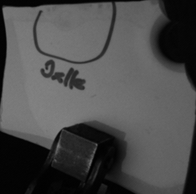
\includegraphics[width = 0.47\textwidth]{04_deflektometrischeRegistrierung/auswertungDeflektometrischeRegistrierung/figures/delleBeleuchtet}
		\caption[Spiegelndes Porzellanbruchstück mit Delle]{Spiegelndes Porzellanbruchstück mit Delle.}
		\label{img:objektMitDelle}
	\end{figure}
}

% Abbildung: Deflektometrische Registrierung bei Objekt mit Delle
{
	\begin{figure}[H]
		\centering
		\begin{adjustbox}{width=\textwidth}
	\begin{tikzpicture}[every node/.style={inner sep=0,outer sep=0}]
	
		\node [anchor=north east] (imgSpalten) at (-0.03\textwidth,0) {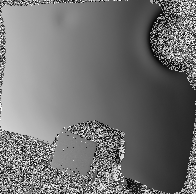
\includegraphics[width=.47\textwidth]{04_deflektometrischeRegistrierung/auswertungDeflektometrischeRegistrierung/figures/spaltenRegistrierung_Delle}};
		\node [below=0.2cm of imgSpalten] {Graubild der Spaltenzuordnung \acrshort{frx}$(x,y)$};
		\node [anchor=north west] (imgZeilen) at (0.03\textwidth,0) {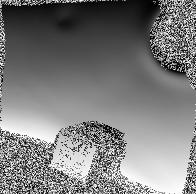
\includegraphics[width=.47\textwidth]{04_deflektometrischeRegistrierung/auswertungDeflektometrischeRegistrierung/figures/zeilenRegistrierung_Delle}};
		\node [below=0.2cm of imgZeilen] {Graubild der Zeilenzuordnung \acrshort{fry}$(x,y)$};
		
	\end{tikzpicture}
\end{adjustbox}
\caption[Deflektometrische Registrierung bei Delle]{Deflektometrische Registrierung des spiegelnden Keramikobjekts aus Abbildung \ref{img:objektMitDelle}.}
		\label{tikz:abbRegistrierungDelle}
	\end{figure}
}

\noindent
In Abbildung \ref{tikz:abbRegistrierungDelle} entsteht im Hintergrund um das Objekt herum eine Störumgebung.
Der Grund dafür ist die fehlende Reflexion des Musters und somit ähnliche Grauwerte in den phasenverschobenen Bildern.
Dies führt dazu, dass in der Bestimmung der Phase $\phi$ für solche Pixel numerisch instabile Ausdrücke und somit schwankende Werte vorkommen.

\p
Die resultierenden Bilder können durch herkömmliche Verfahren aus der Bildverarbeitung weiterverarbeitet und analysiert werden.
Durch die stetigen Grauwertverläufe in den Bildern \acrshort{frx} und \acrshort{fry} an gleichmäßig gekrümmten Oberflächen, lassen sich diese effizient über ihre Ableitungen analysieren (siehe Abbildung \ref{tikz:abbGradientenbildReg}).
Abrupte Änderungen der Grauwerte innerhalb des spiegelnden Objekts führen zu einem höheren Ableitungswert als in der Umgebung. Fehlstellen wie z. B. Dellen oder Pickel lassen sich damit gut detektieren.
Aus demselben Grund erweisen sich auch Hochpassfilterungen als hilfreich \cite{kit_werling}.

% Abbildung: Gradientenbild der deflektometrischen Registrierung.
{
	\begin{figure}[H]
		\centering
		\begin{adjustbox}{width=\textwidth}
	\begin{tikzpicture}[every node/.style={inner sep=0,outer sep=0}]
	
		\node [anchor=north east] (imgSpalten) at (-0.03\textwidth,0) {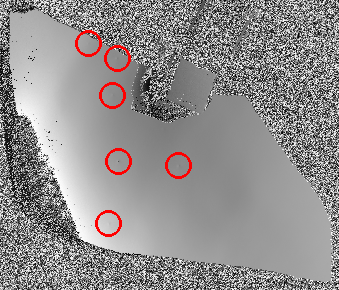
\includegraphics[width=.47\textwidth]{04_deflektometrischeRegistrierung/auswertungDeflektometrischeRegistrierung/figures/pickelDeflektometrischeRegistrierung}};
		\node [below=0.2cm of imgSpalten] {Graubild der Spaltenzuordnung \acrshort{frx}$(x,y)$};
		\node [anchor=north west] (imgGradienten) at (0.03\textwidth,0) {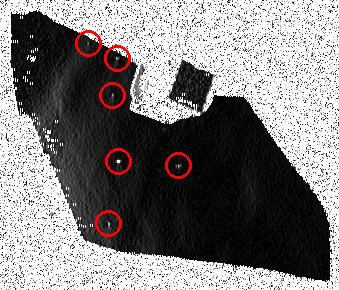
\includegraphics[width=.47\textwidth]{04_deflektometrischeRegistrierung/auswertungDeflektometrischeRegistrierung/figures/pickelGradientenbild}};
		\node [below=0.2cm of imgGradienten, align = center] {Bild der Ableitung von \acrshort{frx}$(x,y)$ \\ in $x$-Richtung};
		
	\end{tikzpicture}
\end{adjustbox}
\caption[Hervorhebung von Pickeln auf reflektierenden Oberflächen.]{Deflektometrische Spaltenregistrierung eines spiegelnden Porzellanbruch\-stücks und das zugehörige Bild der Ableitung. In den rot markierten Stellen lassen sich kleine Abweichungen von einem stetigen Grauwertverlauf erkennen, die in der Ableitung einen Ausschlag haben. Auf dem Prüfobjekt befinden sich an den Stellen kleine Pickel auf der Oberfläche.}
		\label{tikz:abbGradientenbildReg}
	\end{figure}
}

\noindent
Abbildung \ref{tikz:abbGradientenbildReg} zeigt, wie durch die deflektometrische Registrierung kleine Fehlstellen, wie z. B. Pickel auf einer spiegelnden Oberfläche, sichtbar gemacht werden können, die ohne eine spezielle Beleuchtung nicht zu erkennen sind.
Das untersuchte Objekt aus Abbildung \ref{tikz:abbGradientenbildReg} weist am linken Rand vereinzelt matte Stellen auf.
Dadurch treten im Bild der deflektometrischen Registrierung \acrshort{frx} einzelne dunkle Punkte bzw. Artefakte am linken Rand auf.
Diese erkennt man somit auch im Ableitungsbild von \acrshort{frx} als Fehlstellen.

\p
In dem Bild der Ableitung von \acrshort{frx} in $x$-Richtung aus Abbildung \ref{tikz:abbGradientenbildReg} lassen sich Aussagen über die Krümmung der Oberfläche entlang der $x$-Richtung treffen.
Allgemein betrachtet man zu\-nächst eine feste Gerade in der Kameraebene, bezeichnet als Bildkurve.
Die Bildkurve entsteht durch die Spiegelung einer bestimmten Monitorkurve auf einer Oberfläche.
Von der Kurve in der Monitorebene schneiden die ausgehenden Lichtstrahlen die Oberfläche entlang einer Oberflächenkurve.
Über den Zusammenhang der Spiegelabbildung von Geraden und Kurven an gekrümmten Oberflächen lässt sich zeigen, dass die Änderung der Monitorkurve vom linearen Verlauf proportional zur Änderung der Flächennormalen entlang der Oberflächenkurve ist \cite{kit_werling}.
Deutlich wird dies nochmals, wenn man beachtet, dass Geraden bei der Spiegelung nur auf Geraden abgebildet werden können, wenn die Spiegeloberfläche an den Reflexionspunkten einer Ebene entspricht.
Das heißt, dass lokale Änderungen der Tangenten an der Monitorkurve lokalen Abweichungen der Spiegeloberfläche vom ebenen Verlauf entsprechen.
Bekanntlich stellt die deflektometrische Registrierung \acrshort{lr} den Zusammenhang zwischen der Bildebene und der Monitorebene dar.
Demzufolge lässt sich durch das Ableiten der deflektometrischen Registrierung \acrshort{lr} in eine bestimmte Richtung direkt die Abweichung der Flächennormalen, also die wahrgenommene Krümmung der Oberfläche, entlang der Richtung bestimmen.
Die wahrgenommene Krümmung steht in direktem Zusammenhang mit der zweiten Ableitung der Objektoberfläche \cite{kit_werling}.

\p
In Abbildung \ref{tikz:abbGradientenbildReg} erhält man durch die Faltung des Bildes \acrshort{frx} mit Filter für die Ableitung in $x-$-Richtung ein Bild, das in direkter Beziehung zu der Ableitung der deflektometrischen Registrierung \acrshort{lr} in  $x$-Richtung steht.
Somit steht dieses Bild auch im Verhältnis mit der Krümmung der Oberfläche in $x$-Richtung.
Analog lässt sich auch die Krümmung in $y$-Richtung auswerten.

\p
Die deflektometrische Registrierung hat im Vergleich zur Rekonstruktion der Oberfläche essenzielle Vorteile.
Zum Einen kann zur Oberflächenprüfung auf die aufwendige Systemkalibrierung verzichtet werden.
Außerdem ermöglichen die Separierbarkeit und die Darstellung als Bilder den Einsatz von effizienten Methoden aus dem Bereich der Bildverarbeitung.
Das ermöglicht den Einsatz dieser Verfahren für die Erkennung von verschiedenen Fehlstellen auf spiegelnden Oberflächen.
Die Verwendung für transparente Objekte, die Licht durchlassen, ist nur eingeschränkt möglich, da die meiste Information in der Krümmung der Streifenmuster liegt.
Nutzt man also den Monitor als Durchlichtbeleuchtung, ist die Zuordnung trotz vorhandener Fehlstellen überwiegend linear.
Dies kann allerdings auch zum Vorteil genutzt werden, wenn nur diese speziellen Informationen gesucht werden.
}
	}
	
	%Ergebnisse
	{
		\FloatBarrier %Verhindert Fehlpositionierung von Abbildungen aus vorherigen Abschnitten
		\chapter{Ergebnisse}
		\label{chp:ergebnisse}
		Dieses Kapitel beschäftigt sich mit der Analyse und der Bewertung von den eingeführten Verfahren aus den Kapiteln \ref{chp:sichtpruefungDurchLichtstreuung} und \ref{chp:deflektometrischeRegistrierung} zur Auswertung von Oberflächeninformationen spiegelnder und transparenter Prüfobjekte.
	}
	
	%Abschlussbemerkungen
	{
		\FloatBarrier %Verhindert Fehlpositionierung von Abbildungen aus vorherigen Abschnitten
		\chapter{Abschlussbemerkungen}
		\label{chp:abschlussbemerkungen}
		%Zusammenfassung
{
	\FloatBarrier
    \section{Zusammenfassung}
    \label{sec:zusammenfassung}
    Das Ziel dieser Arbeit war es allgemein anwendbare Methoden zur Analyse von spiegelnden und transparenten Oberflächen zu untersuchen, auszuarbeiten und anschließend anzuwenden.
Hierzu wurden zu Beginn der vorliegenden Arbeit die theoretischen Grundlagen der Deflektometrie betrachtet.

\p
Innerhalb der Betrachtungen wurde auf die Ansätze und Möglichkeiten der Deflektometrie eingegangen.
Im Zentrum stand dabei, dass spiegelnde Oberflächen stets über ihre Umgebung wahrgenommen werden müssen und durch geeignete Szenen, die sich auf der Oberfläche spiegeln, Informationen über die Krümmung gewonnen werden können.
Es wurden dabei konkrete Mustersequenzen erklärt, die auf dem heutigen Stand der Technik eingesetzt werden um die Informationen aus der Szene kodiert in den Bildkanal zu übertragen.

\p
Nachdem die deflektometrischen Verfahren zur Rekonstruktion der Objektoberfläche mit ihren Schwierigkeiten und Problemen behandelt wurden, sollten Verfahren zur qualitativen Sichtprüfung dargestellt werden.
Aufgrund weniger zu berücksichtigender Parameter und Einschränkungen sind diese Verfahren besser geeignet für die allgemeine Anwendung.
Durch das bessere Verständnis der Grundlagen konnten im Anschluss Ansätze aufgestellt und Verfahren entwickelt werden, mit denen man die Problemstellung bewältigen kann.
Es wurden zwei Verfahren im Detail beschrieben, um sowohl transparente Objekte, als auch spiegelnde Oberflächen zu untersuchen:
%
\begin{itemize}
	\item Das erste Verfahren wurde in Kapitel \ref{chp:sichtpruefungDurchLichtstreuung} beschrieben. Es werden Streifenmuster verwendet um die abweichende Lichtstreuung an Oberflächendefekten zu nutzen. Im Vergleich zur spiegelnden Oberfläche sind diese Stellen nicht spekular reflektierend. Durch bestimmte Verknüpfungsregeln von Bildern ist es damit möglich die Stellen mit abweichender Lichtstreuung hervorzuheben und daraus Fehlstellen zu erfassen.
	
	\item Das zweite Verfahren wurde in Kapitel \ref{chp:deflektometrischeRegistrierung} beschrieben. Es wird hierbei der Ansatz der Kodierung der Objektoberfläche mithilfe von sinusoidalen Streifenmustern verfolgt. Durch bestimmte Methoden ist es mithilfe von speziellen Mustersequenzen möglich, eine eindeutige Zuordnung von Kamerapunkten und Punkten auf einem Bildschirm bzw. der Szene vorzugeben (deflektometrische Registrierung). Es wurde gezeigt, wie es möglich ist herkömmliche Bildverarbeitungsalgorithmen anzuwenden, um mit der Zuordnung Fehlstellen zu erfassen.
\end{itemize}
%
Diese beiden Verfahren sind zur Anwendung mit in der Bildverarbeitungssoftware NeuroCheck implementiert worden.
Im Anschluss wurden die Ergebnisse der Arbeit an der Implementierung getestet.
Die Tests sollten dazu dienen die Funktionalität der Verfahren und der Implementierung zu prüfen.
Außerdem sollten im Rahmen der Präsentation der Ergebnisse auch die beiden Verfahren für die Anwendung auf spiegelnde und transparente Oberflächen verglichen werden.
Bei den Anwendungen wurden zwei verschiedene Aufbauten gegeneinander getestet (siehe auch Abbildung \ref{tikz:abbAufbauFotos}).
%
\begin{itemize}
	\item Der erste Aufbau umfasste die Auswertung der Bilder durch eine Durchlichtszene. Dies ist nur für transparente Prüfobjekte möglich, da das Objekt zwischen der Szene (ein LCD-Bildschirm) und der Kamera liegt. Die Szenen werden direkt beobachtet und in der Kameraaufnahme durch die transparenten Objekte verzerrt.
	
	\item Der zweite Aufbau umfasste die Auswertung der Bilder durch eine Spiegelbildszene. Dies ist sowohl für spiegelnde, aber auch für transparente Prüfobjekte möglich. Die Szene wird über die Spiegelung auf der Objektoberfläche beobachtet und in der Kameraaufnahme durch die Oberflächenkrümmungen verzerrt.
\end{itemize}
%
Bei den Tests ist deutlich geworden, dass sich für transparente Objekte das erste Verfahren (Sichtprüfung durch Lichtstreuung) sehr gut eignet.
Die besseren Ergebnisse wurden dabei mit dem Durchlichtaufbau erzielt, da der Rückseitenreflex transparenter Objekte mit den vorhandenen Mitteln anders nicht verhindert werden konnte.
Für spiegelnde Oberflächen zeigte Verfahren dieses allerdings Schwächen bei stärkeren Krümmungen und unterschiedlichen Farben auf den Objekten.
Für spiegelnde Objekte ließ sich feststellen, dass das zweite Verfahren (Deflektometrische Registrierung) genauere Ergebnisse liefert hinsichtlich größerer Krümmungen oder unterschiedlichen Farben der Oberflächen.
Außerdem wird es durch die Ergebnisse des Verfahrens möglich tatsächliche Krümmungen der Oberfläche bis zu einer bestimmten Genauigkeit zu erkennen. Hierfür konnte die Ableitung der deflektometrischen Registrierung hinzugezogen werden.

\p
Im Rahmen dieser Arbeit konnte gezeigt werden, dass durch die Beobachtung von Spiegelbildern für spiegelnde Objekte zuverlässig kleinere und größere Oberflächendefekte erfasst werden können.
Für transparente Objekte ist dies auch möglich, allerdings muss das Problem des Rückseitenreflexes dafür gelöst werden. 
Durch die Verwendung des Durchlichtaufbaus war es daher auch möglich Oberflächendefekte zu erfassen.
}

%Ausblick
{
	\FloatBarrier
    \section{Ausblick}
    \label{sec:ausblick}
    Im Ausblick dieser Arbeit stehen mögliche Verbesserungen die an den beschriebenen hier Verfahren vorgenommen werden können.

\p
Ein wichtiger Punkt für die Anwendbarkeit im industriellen Umfeld ist die Laufzeit der Verfahren.
Betrachtet man die Anzahl nötiger Bildaufnahmen zur Bestimmung der deflektometrischen Registrierung, bemerkt man, dass noch Optimierungsbedarf besteht.
Für die Ergebnisse der deflektometrischen Registrierung aus Kapitel \ref{chp:ergebnisse} wurden stets 12 Bildaufnahmen verwendet.
Dabei wurde aber nur die deflektometrische Registrierung der Zeilen betrachtet.
Würde man die vollständige deflektometrische Registrierung bestimmen wollen, so wären dabei 24 Bildaufnahmen nötig gewesen.
Für genauere Messergebnisse können noch weitere Bildaufnahmen hinzugezogen werden.
Eine Überlagerung der sinusoidalen Streifenmuster mit anschließender Trennung im Kamerabild durch eine Fourier-Analyse würde es möglich machen die Anzahl der benötigten Bildaufnahmen für eine vollständige deflektometrische Registrierung um die Hälfte zu reduzieren (vgl. \cite{waveletPMD}).

\p
In Kapitel \ref{chp:ergebnisse} konnte gesehen werden, dass sehr kleine Kratzer oder Laser-Gravuren durch das Bild der deflektometrischen Registrierung nicht sichtbar wurde, dies könnte eine Ungenauigkeit aus der Bilderzeugung sein.
Die Darstellung der Zuordnung als Bild bewirkt, dass eventuell manche Zuordnungen auf denselben Grauwert fallen.
Dies liegt an der mangelnden Anzahl an zu vergebenden Grauwerten.
Durch eine höhere Anzahl an Grauwerten könnte es möglich sein kleinere Oberflächendefekte zu erkennen.
Dies könnte z. B. durch die Verwendung von 16-Bit Informationen für jeden Bildpunkt erreicht werden.

\p
Die Deflektometrie bietet eine große Menge an Verfahren und wird durch stetiger Weiterentwicklung immer genauer und performanter.
Aus dem Grund lassen sich in den beschriebenen Verfahren auch durchaus viele weitere Optimierungsmöglichkeiten finden.
Abschließend lässt sich sagen, dass die deflektometrischen Verfahren vielversprechende Perspektiven bereitstellen um automatisiert spiegelnde oder transparente Oberflächen vollständig zu erfassen und zu prüfen.
}
	}
	
	%Quellenverzeichnis
	{
		\FloatBarrier %Verhindert Fehlpositionierung von Abbildungen aus vorherigen Abschnitten
		\newpage
		\phantomsection
		\addcontentsline{toc}{chapter}{Quellenverzeichnis}
		\printbibliography[title = Quellenverzeichnis]
	}
\end{document}